%\documentclass[12pt, preprint]{aastex}
\documentclass[preprint,times,tighten,linenumbers]{aastex631}

\usepackage{epsf,color,amsmath}

\usepackage{cancel}

\newcommand{\sfrac}[2]{\mathchoice%
  {\kern0em\raise.5ex\hbox{\the\scriptfont0 #1}\kern-.15em/
    \kern-.15em\lower.25ex\hbox{\the\scriptfont0 #2}}
  {\kern0em\raise.5ex\hbox{\the\scriptfont0 #1}\kern-.15em/
    \kern-.15em\lower.25ex\hbox{\the\scriptfont0 #2}}
  {\kern0em\raise.5ex\hbox{\the\scriptscriptfont0 #1}\kern-.2em/
    \kern-.15em\lower.25ex\hbox{\the\scriptscriptfont0 #2}} {#1\!/#2}}

\newcommand{\myhalf}{\sfrac{1}{2}}
\newcommand{\nph}{{n+\myhalf}}
\newcommand{\nmh}{{n-\myhalf}}

\newcommand{\inp}{\mathrm{in}}
\newcommand{\outp}{\mathrm{out}}

% boldsymbol means bold italic
\newcommand{\eb}{{\bf{e}}}
\newcommand{\Ub}{{\bf{U}}}
\newcommand{\xb}{{\bf{x}}}
\newcommand{\kb}{{\bf{k}}}
\newcommand{\Vb}{{\bf{V}}_n}
\newcommand{\Vbhat}{{\bf{\widehat{V}}}_n}
\newcommand{\Omegab}{{\bf{\Omega}}}
\newcommand{\gb}{{\bf{g}}}
\newcommand{\rb}{{\bf{r}}}

\newcommand{\pb}{p_\mathrm{base}}
\newcommand{\epsdot}{\dot{\epsilon}}
\newcommand{\qburn}{q_\mathrm{burn}}
\newcommand{\rt}{\tilde{r}_0}


\newcommand{\nablab}{\mathbf{\nabla}}
\newcommand{\dt}{\Delta\ t}

\newcommand{\omegadot}{\dot{\omega}}

\newcommand{\Hext}{H_{\rm ext}}
\newcommand{\Hnuc}{H_{\rm nuc}}
\newcommand{\kth}{k_{\rm th}}

\newcommand{\Gammaonebar}{\overline{\Gamma}_1}
\newcommand{\Sbar}{\overline{S}}

\newcommand{\etarho}{\eta_\rho}
\newcommand{\etarhoh}{\eta_{\rho~h}}

\newcommand{\Ubt}{\widetilde{\Ub}}
\newcommand{\wt}{\widetilde{w}}

\newcommand{\He}{$^4$He}
\newcommand{\C}{$^{12}$C}
\newcommand{\Fe}{$^{56}$Fe}
\newcommand{\Ni}{$^{56}$Ni}
\newcommand{\Oxygen}{$^{16}$O}


\newcommand{\isot}[2]{$^{#2}\mathrm{#1}$}
\newcommand{\isotm}[2]{{}^{#2}\mathrm{#1}}

\newcommand{\maestro}{{\sf MAESTRO}}
\newcommand{\castro}{{\sf Castro}}
\newcommand{\amrex}{{\sf AMReX}}
\newcommand{\pynucastro}{{\sf pynucastro}}
\newcommand{\microphysics}{{\sf Microphysics}}



\newcommand{\avg}[1]{\overline{#1}}
\newcommand{\avgtwod}[1]{\langle~#1 \rangle}
\newcommand{\rms}[2]{\left(\delta#1\right)_{r_{#2}}}
\newcommand{\mymax}[1]{\left(#1\right)_{\rm max}}

\newcommand{\Tb}{\ensuremath{T_\mathrm{base}}}
\newcommand{\gcc}{\mathrm{g~cm^{-3} }}
\newcommand{\cms}{\mathrm{cm~s^{-1} }}

\newcommand{\half}{\frac{1}{2}}

\setlength{\marginparwidth}{0.5in}

\usepackage{comment}
\usepackage{ulem}

\newcommand{\changeto}[2]{{{\color{red}\sout{#1} }}{{\color{blue} #2}}}
\newcommand{\remove}[1]{{\color{red}\sout{#1}}}
\newcommand{\addto}[1]{{\color{blue} #1}}

\newcommand{\MarginPar}[1]{
    \marginpar{\vskip-\baselineskip%
               \raggedright%
               \tiny\sffamily%
               {\color{red}\hrule%
               \smallskip%
               #1\par%
               \smallskip%
               \hrule}}%
}

\newcommand{\AssignTo}[1]{
    \marginpar{\vskip-\baselineskip%
               \raggedright%
               \tiny\sffamily%
               {\color{blue}\hrule%
               \smallskip%
               #1\par%
               \smallskip%
               \hrule}}%
}

\begin{document}
%======================================================================
% Title
%======================================================================
\title{Sensitivity of He Flames in X-ray Bursts to Nuclear Physics}

\shorttitle{XRB Flame
Sensitivity}
\shortauthors{Chen et al.}

\author[0000-0002-2839-107X]{Zhi Chen}
\affiliation{Department of Physics and Astronomy,
Stony Brook University,
Stony Brook, NY 11794-3800, USA}

\author[0000-0001-8401-030X]{Michael Zingale}
\affiliation{Department of Physics and Astronomy, Stony Brook University,
             Stony Brook, NY 11794-3800, USA}

\author[0000-0001-6191-4285]{Kiran Eiden}
\affiliation{Department of Astronomy,
University of California, Berkeley,
Berkeley, CA 94720-3411, USA}


%% \author[0000-0003-2300-5165]{Donald Willcox}
%% \affiliation{Lawrence Berkeley National Laboratory, Berkeley, CA}

%% \author[0000-0003-0439-4556]{Max P.\ Katz}
%% \affiliation{NVIDIA Corp}

\correspondingauthor{Zhi Chen}
\email{zhi.chen.3@stonybrook.edu}


%======================================================================
% Abstract and Keywords
%======================================================================
\begin{abstract}
Through the use of axisymmetric 2D hydrodynamic simulations, we further investigate laterally propagating flames in X-ray bursts (XRBs). Our aim is to understand the sensitivity of a propagating helium flame to different nuclear physics.  Using the \castro\ simulation code, we confirm the phenomenon of enhanced energy generation shortly after a flame is established after by adding ${}^{12}\mbox{C}(\mbox{p}, \gamma) {}^{13}\mbox{N}(\alpha, \mbox{p}){}^{16}\mbox{O}$ to the network, in agreement with the past literature. This sudden outburst of energy leads to a short accelerating phase, causing a drastic alteration in the overall dynamics of the flame in XRBs. % that is crucial to accurately modeling the flame dynamics in XRBs. 
%We discover that the approximations made in the traditional networks like {\tt aprox13} are still accurate in the context of XRB, but insufficient to correctly model the flame propagation due to the missing rates. 
Furthermore, we investigate the influence of different plasma screening routines on the propagation of the XRB flame. We finally examine the performance of simplified-SDC, a novel approach to hydrodynamics and reaction coupling incorporated in \castro, as an alternative to operator-splitting.


\end{abstract}

\keywords{convection---hydrodynamics---methods: numerical---stars: neutron---X-rays: bursts}

%======================================================================
% Introduction
%======================================================================
\section{Introduction}\label{Sec:Introduction}

An X-ray burst (XRB) is a thermonuclear runaway caused by the ignition of the accreted fuel on the surface of a neutron star. Through Roche-lobe overflow, accreted matter is transferred from the companion star's envelope to the surface of the neutron star. The companion star is likely to have a similar composition to the Sun, i.e.\ a mixture of hydrogen, helium, and a small fraction of carbon, nitrogen, and oxygen \citep{Galloway_2020_basics_of_xrb}. Nuclear explosions are directly affected by the initial composition of the accreted layer and the accretion rate. XRBs found with a mixture of hydrogen and helium fuel layers show bursts with $\sim 5$ sec rise time, while a pure helium layer is typically more explosive and shows bursts with shorter rise times ($\sim 1$ sec). If the shell is enriched with carbon rather than helium, then the explosion is likely to have an extended rise duration, from minutes to hours known as a superburst \citep{Kuulkers_2002,Cumming_2001,Gupta_2007}. 
% This is in contrast to a few seconds in the case of regular type I XRBs, which are XRBs that have a rapid rise time followed by a gradual decline in the light curve. \MarginPar{this last sentence seems redundant}

Since the timescale of accretion between each burst is in the order of $10^4$ secs while the rise time is in the order of $\sim 1 - 10$ sec \citep{Parikh_2013}, it is unlikely for the same thermodynamic condition to exist on the entire surface of the neutron star and for the entire surface to start burning simultaneously \citep{Shara_1982}. Therefore, nuclear ignition is likely to begin in a localized region, and spread to the rest of the neutron star \citep{Spitkovsky_2002}. This asymmetrical burning leads to modulations in the observed flux during the rotation of neutron stars, which causes asymmetrical surface brightness during XRBs \citep{strohmayer_2009}. This explains burst oscillation behavior, a millisecond period variation of XRB intensity during rise time, and the double-peak light curve for non-photospheric-radius-expansion XRBs discovered and supported by observational data \citep{Altamirano_2010,Chakraborty_2014,Bhattacharyya_2006, Kaaret_2007,Smith_1997}.  

% On-sky observations and numerical simulations of XRBs are two approaches for studying the properties of the neutron star and the mechanism of XRBs. Even though there are many successes in constraining the equation of state and the structure of neutron stars through observational data of XRBs \citep{Ozel2016,Nattila2017,lattimer2014constraints,Steiner_2010}, numerical simulations are also critical to assist and complement the study of XRBs and neutron stars due to the limited events of XRBs and the limitations of observational techniques.\MarginPar{not sure we need this sentence justifying why we should do simulations}

Numerous successful numerical simulations have explored the properties of neutron stars and XRBs.
One-dimensional simulations can determine the nucleosynthesis, study the rp-process, estimate burst duration, and predict the light curve of XRBs by assuming spherical symmetry \citep{Woosley_2004,Johnston_2018,Meisel_2018,Johnston_2020}. On the other hand, multi-dimensional simulations are conducted to study the behavior of lateral flame propagation and flame structure for their nontrivial contributions to the structure of the XRB light curve \citep{eiden:2020,harpole:2021,cavecchi:2013,Cavecchi_2015,Cavecchi_2016}.

% Propagating flames can be classified into two categories, detonation and deflagration. Detonation XRB models \cite{Zingale_2001} were conducted in the early times since they're relatively computationally inexpensive. However, deflagration models are more accurate and realistic because detonation is only likely to occur with extreme thermodynamical conditions (A cite here probably). 

% The effect of Coriolis force on the spread of the deflagrating nuclear flame was investigated in \cite{cavecchi:2013} to demonstrate the dependence of rotational frequency, $\nu$ and heat conductivity of the fluid, $\kappa_c$, on the flame speed as $1/(\nu \sqrt{\kappa_c})$. \cite{Cavecchi_2015} showed that flame can pass the equator if the flame originated from the pole. It also showed the differences in flame propagation depending on the origin and the destination (from pole to equator vs. from the equator to pole) on the neutron star. The effect of the magnetic field and its interaction with the Coriolis force on flame propagation is explored in \cite{Cavecchi_2016}. It is discovered that a strong magnetic field can effectively slow down the flame speed, while a weak magnetic field can cause the flame to travel at a faster speed compared to no magnetic field at all. 

In our first work, \cite{eiden:2020}, we studied the overall behavior of the burning front propagation using a 2D simulation with various approximations like artificially boosted flame speed and simple networks to minimize the computational cost, as well as high rotation rate to reduce the lateral flame length scale for greater flame confinement. In \cite{harpole:2021}, we continued our work to explore the effect of rotation rate and crust temperature on flame propagation. We discovered that flame propagation was not greatly affected by the rotation rate, which is likely due to the balance between the confinement of the flame and the enhanced nuclear reaction rates caused by the increased rotation rate. It is also demonstrated that a cooler crust temperature drives a reduced flame speed and vice versa. 
Finally, in \citet{xrb_flame_3d} we showed
that 2D axisymmetric simulations compare well to full 3D simulations in capturing the nucleosynthesis of the early flame propagation.
Continuing our work, we investigate the effects of different reaction networks, plasma screening methods, and time integration methods on the simulation of lateral flame propagation in XRBs. 

%======================================================================
% Numerical Approach
%======================================================================
\section{Numerical Approach}\label{Sec:numerics}
% Here briefly describe castro and the physics

We use {\castro} \citep{castro,castro_joss}, an open-source, adaptive mesh, astrophysical simulation code, to perform all the simulations discussed in this manuscript. The reaction networks,
integrators, equation of state \citep{timmes_swesty:2000}, thermal neutrino losses \citep{neutrino}, and conductivities
\cite{Timmes00} are contained in the related {\microphysics} package \citep{starkiller}. 

Our simulation setup is the same as described in \citep{eiden:2020, harpole:2021}, so here we only reiterate the essential points. The simulations are performed using a 2D r-z cylindrical geometry, assuming azimuthal symmetry. 
The hydrodynamics is evolved using an unsplit piecewise parabolic method \citep{ppm,ppmunsplit,millercolella:2002}.
We work with a corotating frame, and assume a rotational frequency $\Omega = 1000$ Hz for the neutron star.  Gravity is assumed to be constant, since the accreted layer is thin.  Our initial model is also unchanged from our previous papers.  We employ a hydrostatic initial model to represent the neutron star's initial thermodynamic conditions, with a hot model in the left part of the domain and a cool model in the right---this drives a rightward propagating flame (a spreading hotspot for our geometry).  By default, reactions are incorporated using
operator-splitting.

%the atmosphere divided into distinct regions based on height, $z$. The isothermal base region ($0 < z < H_*$) represents the underlying neutron star and consists of the pure ${}^{56}$Ni with a temperature of $T_*$. The hyperbolic tangent transition phase ($H_* < z < H_* + 3 \delta_{\textrm{atm}}$) is characterized by a prescribed temperature and composition profile that transitions from the base region to the pure ${}^{4}$He isentropic atmosphere. The isentropic atmosphere ($z > H_* + 3 \delta_{\textrm{atm}}$) is solved for the corresponding temperature and density, subject to the hydrostatic and isentropic constraints, with the minimum temperature and density set as $T_{\textrm{lo}}$ and $\rho_{\textrm{cutoff}}$, respectively. The prescribed hyperbolic tangent transition profile on the left side of the domain ($r < r_{\textrm{pert}}$) is higher than the other side ($r > r_{\textrm{pert}}$), representing the initial temperature perturbation where the thermonuclear flame initiates.


This paper investigates the effect of reaction networks on the flame.  We explore four different networks including a standard 13-isotope alpha chain as our reference network (see Sec.\ \ref{Sec:network}), two
different plasma screening implementations (Sec.\ \ref{Sec:screening}), and how the reactions and hydro are coupled
together (Sec.\ \ref{Sec:integration}).


\begin{comment}
We use {\castro} \citep{castro,castro_joss}, an adaptive mesh, astrophysical radiation hydrodynamics simulation code, to perform all the simulations discussed in this manuscript. {\castro} evolves a general system of fully-compressible Euler's equations:

\begin{align}
    \frac{\partial \rho}{\partial t} + \nabla \cdot (\rho \mathbf{U}) &= S_{\textrm{ext},\rho} \label{Eq:castro_mass}\\
    \frac{\partial (\rho \mathbf{U})}{\partial t} + \nabla \cdot (\rho \mathbf{U}\mathbf{U}) + \nabla p &= S_{\textrm{ext},\rho \mathbf{U}} \label{Eq:castro_momen}\\
    \frac{\partial (\rho E)}{\partial t} + \nabla \cdot (\rho \mathbf{U} E + \rho E)  &= \nabla \cdot k_{\textrm{th}} \nabla T +\rho \dot{\epsilon} + S_{\textrm{ext}, \rho E} \label{Eq:castro_energy} \\
    \frac{\partial(\rho X_k)}{\partial t} + \nabla \cdot (\rho \mathbf{U}X_k) &=  \rho \dot{\omega}_k + S_{\textrm{ext}, \rho X_k} \label{Eq:castro_massfrac}
\end{align}

where $\rho$ is the density, $\mathbf{U}$ is the velocity vector, $p$ is the pressure, $X_k$ is the nuclei mass fraction with the constraint $\sum_k X_k = 1$, and $E$ is the total energy per unit mass, which can be related to the internal energy per unit mass, $e$, and the kinetic energy per unit mass as $e = E -  |\mathbf{U}|^2 / 2$. This system of equations are closed by supplying the Equation of State (EOS) such that $p = p(\rho, e, X_k)$. We follow the same convention introduced in \cite{eiden:2020}, where $(r, z, \theta)$ coordinate system is used instead of the traditional cylindrical coordinate system. Therefore, the velocity vector, $\mathbf{U}$, is now decomposed into $(u, v, w)$, where positive $w$ represents the velocity in the $\theta$ direction pointing out of the page. Thermal diffusion is modelled by incorporating an explicit source term, $\nabla \cdot k_{\textrm{th}} \nabla T$, characterized by the thermal conductivity, $k_{\textrm{th}}$, and temperature, $T$, into the energy equation (Eq. \ref{Eq:castro_energy}). The change in reacting isotopes is characterized by $\dot{\omega}_k$, the creation rates for the $k$-th isotope. The energy input term from the nuclear burning process, $\rho \dot{\epsilon}$, is added to the energy equation where $\dot{\epsilon}$ is the specific energy generation rate. Lastly, $S_{\textrm{ext}}$ represents all possible external sources terms.

In this manuscript, the same setup is used and discussed in our previous XRB papers \cite{eiden:2020, harpole:2021}. A detailed description is provided in \cite{eiden:2020}, and here we only reiterate the essential points. The simulation is performed using a 2D r-z cylindrical coordinate system by assuming azimuthal symmetry. It is convenient to work with a co-rotating frame since we're working with a rotating neutron star, which introduces Coriolis force term, $ -2\rho \mathbf{\Omega} \times \mathbf{U}$, to Euler's equation along with the gravity term, $\rho \mathbf{g}$.
%In general, the gravitational acceleration, $\mathbf{g}$, is found by solving the Poisson equation, $\nabla^2 \Phi = 4\pi G \rho$, where $\mathbf{g} = -\nabla\Phi$. 
We considered a constant gravity, $\mathbf{g}$. Considering the timescale of the XRB, the angular velocity is set to be fixed in the z-axis, $\mathbf{\Omega} = \Omega_0 \hat{z}$ to avoid extra source ter, $- \rho d\mathbf{\Omega}/dt \times \mathbf{r}$. The centrifugal force, $- \rho \mathbf{\Omega} \times (\mathbf{\Omega} \times \mathbf{r})$, is also neglected for the simplicity of the problem.
We also added geometric source terms, $\frac{1}{r}\rho w^2 \hat{r} - \frac{1}{r}\rho uw \hat{\theta}$, suggested by \cite{BERNARDCHAMPMARTIN2013170}, which arise from applying the cylindrical divergence term, $\nabla \cdot (\rho \mathbf{U}\mathbf{U})$ in Eq. \ref{Eq:castro_momen} for axisymmetric geometry.

Finally, we incorporated a density sponge mechanism \citep{ABNZ:III, Malone2014a,xrb2} with the objective of reducing the fluid velocity in the initial phase of the simulation when the flame is being established. This helps prevent the violent ejection of materials that can create unnecessary timestep constraints when studying flame propagation. The sponge mechanism adds an extra damping external source term, $\rho \mathbf{U} f/\Delta t$ and $\rho \mathbf{U}^2 f/\Delta t$, to the momentum and energy equations, where $f$ is the density dependent damping coefficient that equals to 0 once $\rho > 10^2 \ \mathrm{g} \ \mathrm{cm}^{-3}$ and $\Delta t$ is the timestep. The sponge mechanism is designed so that the damping mechanism has a greater damping effect when $\tau_{\mathrm{sponge}} < \Delta t$ with $\tau_{\mathrm{sponge}} = 10^{-7} $ s. The overall external source terms for our current setup is the following: 

\begin{subequations}\label{Eq:castro_source}
\begin{equation}
    S_{\textrm{ext},\rho} = 0
\end{equation}

\begin{equation}
    S_{\textrm{ext},\rho \mathbf{U}} = -2\rho \mathbf{\Omega} \times \mathbf{U} + \frac{1}{r}\rho w^2 \hat{r} - \frac{1}{r}\rho uw \hat{\theta} + \rho \mathbf{g} + \rho \mathbf{U} \frac{f}{\Delta t}
\end{equation}

\begin{equation}
    S_{\textrm{ext}, \rho E} = \rho \mathbf{U} \cdot \mathbf{g} + \rho |\mathbf{U}|^2 \frac{f}{\Delta t}
\end{equation}

\begin{equation}
    S_{\textrm{ext}, \rho X_k} = 0. 
\end{equation}
\end{subequations}

Here we re-emphasize that Coriolis force plays an important role at limiting the horizontal length scale for flame confinement suggested by \cite{Spitkovsky_2002}. It can be shown that \citep{eiden:2020} the momentum equation (Eq. \ref{Eq:castro_momen}) has an explicit $w$ component, Eq. \ref{Eq:w_term}, a simple advection equation with the source term, $2 \Omega_0 u$ that is also solved during the simulation.

\begin{equation}\label{Eq:w_term}
    \frac{\partial w}{\partial t} + \mathbf{U} \cdot \nabla w = 2\Omega_0 u.
\end{equation}

The overall nuclear burning process is incorporated using the {\microphysics} \citep{starkiller} package. {\sf Helmholtz} EOS, a general EOS based on a table interpolation of the Helmholtz free energy described in \cite{timmes_swesty:2000}, is used. A general routine described in appendix A of \cite{Timmes00} is used to model thermal conductivity. We follow the procedure described in \cite{neutrino} to model thermal neutrino losses.

We selected 4 different reaction networks to study the dependence of reaction networks on the laterally propagating flame. We used the {\tt aprox13} network as the reference network for comparison with the other 3 networks. The details of these reactions networks are discussed in Sec. \ref{Sec:network}. We used two different plasma screening routines, {\tt SCREEN5} and {\tt CHUGUNOV2007}, to model plasma screening strengthening effects on the reaction rates. The details of the two screening methods are discussed in Sec. \ref{Sec:screening}. The RHS of the network is automatically generated using {\pynucastro} \citep{pynucastro, pynucastro2, the_pynucastro_development_2022_7239007} and ported to {\microphysics}. The RHS of the network is then solved along with the EOS, plasma screening method, thermal conductivity, and neutrino loss using VODE \citep{vode} in {\microphysics}. Lastly, the coupling between hydrodynamics and nuclear reactions are performed via either Strang-splitting \citep{strang:1968} or the simplified SDC approach \citep{Zingale_2022}. The details of these time integration methods are discussed in Sec. \ref{Sec:integration}. 


{\castro} uses the adaptive mesh refinement system from {\amrex} \citep{amrex_joss}. The same simulation domain of $r = 1.8432 \times 10^5$ cm and $z = 3.072 \times 10^4$ cm is used for all of our models. At the coarse grid, we again used $1152 \times 192$ zones with two additional refinement levels with refinement ratios of 4 and 2. This means that the first refinement level is 4 times finer than the coarse level and the finest level is 2 times finer than the first level. This enables us to achieve a finest level with $9216 \times 1536$ zones, corresponding to a resolution of 20 cm. Grid refinement is limited to regions where $\rho > 2.5 \times 10^4 \ \textrm{g} \ \textrm{cm}^{-3}$ in order to avoid unncessary computational costs.

A complete description of the simulation domain necessitates the specification of a set of boundary conditions. For the left boundary, $r=0$, we have employed a symmetry or reflecting boundary condition. This choice ensures that the normal velocity of the fluid on the other side of the boundary has an opposite sign, allowing for laterally propagating flame from $z=0$. An outflow boundary condition is implemented for the right boundary. For the bottom boundary, we have employed a hydrostatic equilibrium (HSE) boundary condition described in \cite{ppm-hse}, which ensures that the HSE condition of the last interior zone of the boundary is integrated to the ghost cell. The ghost cells at the bottom of the simulation domain have a constant temperature of  $T= 1 \times 10^8$ K, consistent with the temperature of the neutron star. Moreover, the normal velocity at the bottom boundary is reflected with a zero-gradient transverse velocity. Finally, an ambient-fill boundary condition has been employed along with a standard normal velocity outflow for the top boundary. This boundary condition utilizes the initial model conditions and allows for a zero-gradient outflow for the velocity.

\subsection{Initial Models}\label{Sec:models}
% Here describe the initial setup of the problem.
% Show initial profiles?

This study begins by characterizing the atmospheric structure and initial thermodynamic conditions of the neutron star before the burning process begins. The initial model used in this simulation is identical to the ones used in our previous papers, and is discussed in detail in \cite{eiden:2020}. To construct the initial model, two 1D hydrostatic atmospheric vertical profiles are created as a function of $z$ to represent temperature-perturbed and unperturbed regions. These profiles incorporate both isentropic and isothermal conditions. The next step is to blend these two profiles as a function of $r$, resulting in the final initial model as a function of $(r,z)$. For this manuscript, we assume a pure ${}^{4} \mathrm{He}$ fuel layer on the surface of the star with a pure ${}^{56} \mathrm{Ni}$ core. Table \ref{Tab:initial_model} lists all input parameters.


\begin{table*}
\caption{\label{Tab:initial_model}
Input parameters for constructing the initial model.
}
\begin{ruledtabular}
\begin{tabular}{cc}
Input Parameters &
Values
\\ 
\colrule

$\mathbf{\Omega}$ & 1000 Hz $\hat{z}$\\
$T_*$    & $10^8$ K \\
$T_{\mathrm{hi}}$  & $2 \times 10^8$ K \\
$T_{\mathrm{lo}}$  & $8 \times 10^6$ K \\
$\delta T$  & $1.2 \times 10^9 $ K \\
$r_{\mathrm{pert}}$  & $4.096 \times 10^4$ cm \\
$\delta_{\mathrm{blend}}$ & 2048 cm \\
$\rho_{\mathrm{base}}$ & $3.43 \times 10^6 $ $\mathrm{g \ cm^{-3}}$ \\
$H_*$  & 2000 cm \\
$\delta_{\mathrm{atm}}$ & 50 cm \\
$X_{k_{\mathrm{base}}}({}^{56} \mathrm{Ni})$ & 1.0 \\
$X_{k_{\mathrm{fuel}}}({}^{4} \mathrm{He})$ & 1.0 \\
$\rho_{\mathrm{cutoff}}$ & $10^{-4}$  $\mathrm{g \ cm^{-3}}$ \\
$\mathbf{g}$ & $-1.5\times 10^{14}$ $\mathrm{g \ s^{-2}}$ $\hat{z}$\\
 
\end{tabular}
\end{ruledtabular}
\end{table*}

To generate the 1D atmospheric profile, we first define the base of neutron star for $z < H_*$, where $H_*$ denotes length scale of the base layer. 
Subsequently, we set the initial temperature and composition profiles, contingent upon whether $z > H_*$ or $z < H_*$. For the atmosphere region, $z > H_*$, both the temperature and composition follow a hyperbolic tangent transition that follows Eq. \ref{Eq:tanh-eqs}. In this equation, $T_*$ represents the temperature of the star, $T_{\mathrm{hi}}$ represents the highest temperature of the profile, $X_{k_{\mathrm{fuel}}}$ represents the mass fractions of the fuel layer, $X_{k_{\mathrm{base}}}$ represents the mass fractions of the base layer, and $\tilde{z} = z - H_* - 3/2 \delta_{\mathrm{atm}}$, where $\delta_{\mathrm{atm}}$ denotes a characteristic length scale. For the base region, $z < H_*$, a uniform temperature and composition profile is used, where $T = T_*$ and $X_k = X_{k_{\mathrm{base}}}$. Initially, the density and pressure for all regions are set to be the values at the base, $\rho = \rho_{\mathrm{base}}$ and $p = p_{\mathrm{base}}$, where pressure at the base, $p_{\mathrm{base}}$, is determined via EOS. These steps complete our preliminary description of the profile.


\begin{subequations}\label{Eq:tanh-eqs}

\begin{equation}
    T(z) = T_* + \frac{1}{2}\left(T_{\mathrm{hi}} - T_*\right)\left[1 + \tanh{\left( \frac{2\tilde{z}}{\delta_{\mathrm{atm}}} \right)}\right]
\end{equation}

\begin{equation}
    X_k(z) = X_{k_{\mathrm{fuel}}} + \frac{1}{2}\left(X_{k_{\mathrm{base}}} - X_{k_\mathrm{fuel}}\right)\left[1 + \tanh{\left( \frac{2\tilde{z}}{\delta_{\mathrm{atm}}} \right)}\right]
\end{equation}

\end{subequations}

We used the discretized HSE equations, Eq. \ref{Eq:hse_up} and \ref{Eq:hse_down}, to integrate the HSE states of the star starting from the base at $z=H_*$. Eq. \ref{Eq:hse_up} calculates the pressure at the current zone, $p_i$, by assuming that the pressure from the previous zone, $p_{i-1}$, is known and integrating upwards. Conversely, Eq. \ref{Eq:hse_down} follows a similar process by integrating downwards to obtain the pressure at the current zone, $p_i$, with the assumption that the pressure at the subsequent zone, $p_{i+1}$ is known. Using the HSE condition described in Eq. \ref{Eq:hse_up}, we perform Newton-Raphson iterations to obtain HSE states by integrating upwards from $z = H_*$. An isothermal profile is employed when $H_* < z < H_* + 3 \delta_{\mathrm{atm}}$. In this region, the initial temperature profile is held constant and only density is solved for, subject to the HSE constraint. The entropy and pressure are both updated using the EOS. At $z = H_* + 3 \delta_{\mathrm{atm}}$, the entropy, $s$, provides an additional constraint for the isentropic atmosphere profile. This is the region in which the hyperbolic tangent transition phase for temperature occurs.

\begin{subequations}
\begin{equation}\label{Eq:hse_up}
    p_i = p_{i-1} + \frac{1}{2}\Delta z( \rho_i + \rho_{i-1})\mathbf{g} \cdot \hat{\mathbf{z}}
\end{equation}

\begin{equation}\label{Eq:hse_down}
    p_i = p_{i+1} + \frac{1}{2}\Delta z( \rho_i + \rho_{i+1})\mathbf{g} \cdot \hat{\mathbf{z}}
\end{equation}
\end{subequations}

When $z > H_* + 3\delta_{\mathrm{atm}}$, the atmosphere transitions to an isentropic state which provides an additional entropy constraint, allowing for solving both density and temperature. However, when  $T < T_{\mathrm{lo}}$, another isothermal region is established. In this region, a uniform profile of $T = T_{\mathrm{lo}}$ is employed, while density is still solved for. As the atmosphere becomes thinner such that $\rho < \rho_{\mathrm{cutoff}}$, a constant profile of $\rho = \rho_{\mathrm{cutoff}}$ and $T = T_{\mathrm{lo}}$ is used. Once the atmosphere profile for $z > H_*$ is fully determined, we integrate downwards from $z = H_*$ using Eq. \ref{Eq:hse_down} as the constraint equation to update states in the base region. The base region is defined entirely using an isothermal profile, with density being determined by setting $T = T_*$. Different regions of the 1D hydrostatic model can then be summarized into the following:

\begin{enumerate}
    \item an isothermal base with $T = T_*$ when $0 < z < H_*$.
    \item a transition phase with prescribed temperature and composition profiles that blend the base and the atmosphere when $ H_* < z < H_* + 3\delta_{\mathrm{atm}}$.
    \item an isentropic atmosphere for flame propagation when $z > H_* + 3\delta_{\mathrm{atm}}$, $T > T_{\mathrm{lo}}$ and $\rho > \rho_{\mathrm{cutoff}}$.
    \item an isothermal low temperature buffer region when $T < T_{\mathrm{lo}}$.
    \item an isothermal and constant low density buffer region when $\rho < \rho_{\mathrm{cutoff}}$.
\end{enumerate}

The 2D initial model is obtained by combining two 1D hydrostatic vertical profiles, one representing the ``hot" model with temperature perturbations, and the other representing the ``cold" model with unperturbed-thermodynamic conditions. The construction of both models follows the description provided above, with the only difference being that $T_{\mathrm{hi}}$ is replaced with $T_{\mathrm{hi}} + \delta T$ in the ``hot" model. The ``hot" model is placed at $r < r_{\mathrm{pert}}$, where the flame is expected to start, while the ``cold" model is placed at  $r > r_{\mathrm{pert}} + \delta_{\mathrm{pert}}$. A smooth linear transition region, $r_{\mathrm{pert}} \leq r \leq r_{\mathrm{pert}} + \delta_{\mathrm{pert}}$, exists between the two models, characterized by $\delta_{\mathrm{pert}}$, which represents the length scale of the transition region. Finally, the EOS is called to update all thermodynamic quantities within the transition region. 
\end{comment}


% The blending process is described by Eq. \ref{Eq:blend}, where $r_{\mathrm{perturbed}} = 4.096 \times 10^4$ cm and the blending length scale, $\delta_{\mathrm{pert}} = 2048$ cm.

% \begin{subequations}\label{Eq:blend}
% \begin{equation}
%     f(r) = 1 - \frac{r - r_{\mathrm{pert}}}{\delta_{\mathrm{blend}}}
% \end{equation}

% \begin{equation}
%     \mathcal{Q}(r, z) = \left\{\begin{array}{lr}
%          \mathcal{Q}_{\mathrm{hot}}(z)  & \quad r < r_{\mathrm{pert}} \\
        
%         f(r)\mathcal{Q}_{\mathrm{hot}}(z) + \left[1 - f(r)\right]\mathcal{Q}_{\mathrm{cool}}(z) & \quad r_{\mathrm{pert}} \leq r \leq r_{\mathrm{pert}} + \delta_{\mathrm{pert}}\\
        
%         \mathcal{Q}_{\mathrm{cool}}(z)  & \quad r > r_{\mathrm{pert}} + \delta_{\mathrm{pert}}
%         \end{array}\right\}, \quad\mathcal{Q} \in \{p, \rho, X_k\}
% \end{equation}
% \end{subequations}


\subsection{Nuclear Reaction Networks}\label{Sec:network}
% Discuss APROX13, subch_full, subch_full_with_2rates_turned_off, subch_simple

During an XRB, nucleosynthesis involves more than a thousand isotopes \citep{Woosley_2004,Koike_2004}. However, due to computational constraints, most multi-dimensional simulations incorporate fewer than 20 isotopes. Thus, this paper aims to understand how the different approximations used in the nuclear physics impact on the lateral thermonuclear flame in XRBs.

\subsubsection{\tt aprox13}

In \citet{eiden:2020,harpole:2021}, we used the 13-isotope $\alpha$-chain network, {\tt aprox13} \citep{timmes_aprox13} network.  We'll
use that as the reference network for comparison here.  
%Visuals can be found in Figure \ref{fig:networks}. 
The main feature of {\tt aprox13} is the $(\alpha, \mbox{p})(\mbox{p}, \gamma)$ approximation that eliminates the intermediate nuclei involved in $(\alpha, \mbox{p})(\mbox{p}, \gamma)$ by
assuming proton equilibrium in the reactive flow.
As a result, {\tt aprox13} has a total of 13 isotopes and 31 rates. Nevertheless, the $(\alpha, \mbox{p})(\mbox{p}, \gamma)$ approximation can become less accurate for temperatures $\gtrsim 2.5 \times 10^9$ K, potentially affecting the energy generation rates.  An illustration of this can be found in \cite{pynucastro2} (see Figure 6 there).

% Figure \ref{fig:aprox_comparison} depicts the evolution of the 13 {\tt aprox13} species under constant thermodynamic conditions, $\rho = 10^6$ g $\mathrm{cm}^{-3}$ and $T = 2 \times 10^9$ K. The solid lines represent the evolution with the $(\alpha, \mbox{p})(\mbox{p}, \gamma)$ approximation, while the dashed lines do not include this approximation. At $T = 2 \times 10^9$ K, we observe minor differences in the mass fractions of the heavier species (${}^{36}$Ar, ${}^{40}$Ca, ${}^{44}$Ti, ${}^{48}$Cr) that involved in $(\alpha, \mbox{p})(\mbox{p}, \gamma)$ approximation. 


% \begin{figure}
% \centering
% \plotone{aprox_comparison.pdf}
% \caption{\label{fig:aprox_comparison} A comparison of the evolution of 13 species in {\tt aprox13} with and without $(\alpha, \mbox{p})(\mbox{p}, \gamma)$ approximation. The solid lines and the dashed lines show the evolution with and without  $(\alpha, \mbox{p})(\mbox{p}, \gamma)$ approximation, respectively. The RHS of the mass fractions are obtained using the {\pynucastro} package and integrated with $\rho = 10^6$ g $\mathrm{cm}^{-3}$ and $T = 2.0 \times 10^9$ K.}
% \end{figure}

% \MarginPar{I think for this figure, we can just refer to the similar one in the pynucastro paper}

As XRBs can reach temperatures close to the aforementioned limit ($T \gtrsim 2.5\times 10^9$ K), it important to
understand if this approximation affects the flame.  Therefore, we employ three more intricate networks, built with \pynucastro\ using the latest rates from the {\sf REACLIB} \citep{reaclib} library.  These networks are described below. 


\subsubsection{{\tt subch\_full} and {\tt subch\_full\_mod}}

The {\tt subch\_full} network was introduced in Appendix B of \cite{castro_simple_sdc} for simulating He burning in sub-Chandrasekhar mass white dwarfs (hence, the {\tt subch} prefix). {\tt subch\_full} network has three main modifications compared to {\tt aprox13} network. First {\tt subch\_full} explicitly includes the intermediate nuclei for the $(\alpha, \mbox{p})(\mbox{p}, \gamma)$ sequence.  Second, it has
a better representation of carbon and oxygen burning by including the endpoint nuclei of the difference branches: ${}^{12}\mbox{C}({}^{12}\mbox{C}, \mbox{p}) {}^{23}\mbox{Na} (\mbox{p}, \gamma) {}^{24}\mbox{Mg}$, ${}^{12}\mbox{C} ({}^{12}\mbox{C}, \mbox{n}){}^{23}\mbox{Mg} (\mbox{n}, \gamma) {}^{24}\mbox{Mg}$,  ${}^{16}\mbox{O} ({}^{16}\mbox{O}, \mbox{n}){}^{31}\mbox{S} (\mbox{n}, \gamma) {}^{32}\mbox{S}$, and ${}^{16}\mbox{O} ({}^{12}\mbox{C}, \mbox{n}){}^{27}\mbox{Si} (\mbox{n}, \gamma) {}^{28}\mbox{Si}$.  Since the neutron capture processes on the intermediate nuclei happen at a fast timescale, the rates
including neutrons are approximated by assuming the subsequent neutron capture is instantaneous as ${}^{12}\mbox{C} ({}^{12}\mbox{C}, \gamma) {}^{24}\mbox{Mg}$,  ${}^{16}\mbox{O} ({}^{16}\mbox{O}, \gamma) {}^{32}\mbox{S}$, and ${}^{16}\mbox{O} ({}^{12}\mbox{C}, \gamma) {}^{28}\mbox{Si}$, and the network does not include neutrons. We also note that their reverse rates are not included due to their negligible effects at $T \sim 10^9$ K.  Finally, we included the additional rates ${}^{14}\mbox{N}(\alpha,\gamma){}^{18}\mbox{F}(\alpha, \mbox{p}){}^{21}\mbox{Ne}$ and ${}^{12}\mbox{C}(\mbox{p}, \gamma) {}^{13}\mbox{N}(\alpha, \mbox{p}){}^{16}\mbox{O}$, discussed in \cite{Shen_2009, Weinberg_2006,Karakas_2008, fisker:2008} to bypass the comparatively slow ${}^{12}$C $\alpha$-capture process, ${}^{12}\mbox{C} (\alpha, \gamma) {}^{16}\mbox{O}$, when $T \gtrsim 10^9$ K. The first $\alpha$-capture process on ${}^{14}\mbox{N}$ and ${}^{18}\mbox{F}$ led to the production of protons that can be used for the $\alpha$ chain process on ${}^{12}\mbox{C}$. When $T \gtrsim 10^9$ K, ${}^{12}\mbox{C}(\mbox{p}, \gamma) {}^{13}\mbox{N}(\alpha, \mbox{p}){}^{16}\mbox{O}$ is expected to dominate the reactive flow towards the heavy $\alpha$ chain nuclei, which can lead to a completely different end-stage composition \citep{Weinberg_2006, fisker:2008}. Since these additional rates leave ${}^{21}\mbox{Ne}$ as the endpoint, ${}^{22}\mbox{Na}$ is added to connect all the nuclei. With all the modifications, {\tt subch\_full} has 28 isotopes and 107 rates. 
Figure~\ref{fig:networks} shows a visualization
of this network.

{\tt subch\_full\_mod} is identical to the {\tt subch\_full} network, except that the ${}^{12}\mbox{C}(\mbox{p}, \gamma) {}^{13}\mbox{N}(\alpha, \mbox{p}){}^{16}\mbox{O}$ and its reverse reactions are turned off. This is done to explore the significance of these two rates, as described in \cite{Shen_2009, Weinberg_2006, fisker:2008}. 

\begin{comment}
This gives {\tt subch\_full\_mod} 27 isotopes and 103 rates in total. The second and third panel of Figure \ref{fig:networks} gives an overview of {\tt subch\_full} and {\tt subch\_full\_mod} networks. Here we note that \cite{Shen_2009} also discussed that the $\alpha$-capture chain, ${}^{14}\mbox{C}(\alpha,\gamma){}^{18}\mbox{O}(\alpha,\gamma){}^{22}\mbox{Ne}$, will take place at temperatures $\gtrsim 10^9$ K. However, this process is currently not considered since the energy contribution from this rate is likely to be negligible due to the small abundance of ${}^{14}\mbox{C}$ during nucleosynthesis. 
\end{comment}

\subsubsection{\tt subch\_simple}

Lastly, we present {\tt subch\_simple} network, a simplification of {\tt subch\_full} network that would resemble a more similar network to {\tt aprox13}. The network omits a total of six nuclei, namely ${}^{35}\mbox{Cl}$, ${}^{39}\mbox{K}$, ${}^{43}\mbox{Sc}$, ${}^{47}\mbox{V}$, ${}^{51}\mbox{Mn}$, and ${}^{55}\mbox{Co}$, using the $(\alpha, \mbox{p})(\mbox{p}, \gamma)$ approximation. The reverse rates of all ${}^{12}\mbox{C} + {}^{12}\mbox{C}$,  ${}^{16}\mbox{O} + {}^{16}\mbox{O}$, and ${}^{16}\mbox{O} + {}^{12}\mbox{C}$ are removed since they are not present in {\tt aprox13}. 
All the forward and reverse rates of ${}^{12}\mbox{C} + {}^{20}\mbox{Ne}$ , ${}^{23}\mbox{Na}(\alpha, \gamma){}^{27}\mbox{Al}$, and ${}^{27}\mbox{Al}(\alpha, \gamma){}^{31}\mbox{P}$ are also removed to simplify the network.
After the simplifications, we now have 22 isotopes and 57 rates. See the bottom panel of Figure \ref{fig:networks} for visualization.

\begin{figure}
\centering
%\plotone{aprox13.pdf}
\plotone{subch_full.pdf}
%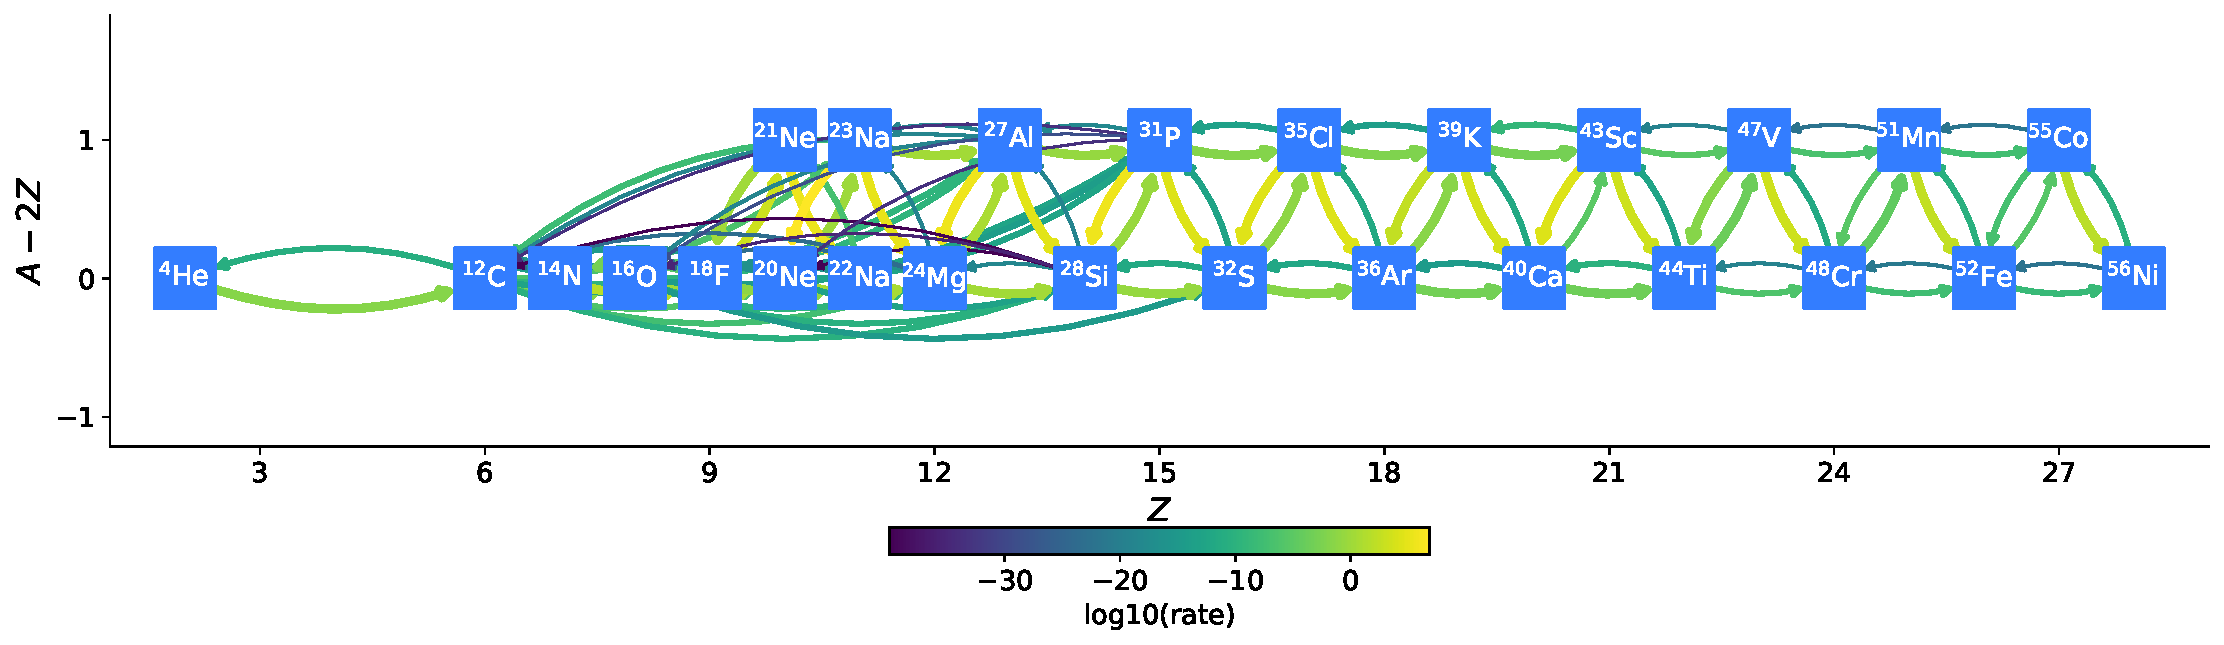
\includegraphics[width=0.88\linewidth]{subch_full_mod.pdf}
\plotone{subch_simple.pdf}
\caption{\label{fig:networks} A simple visualization {\tt subch\_full} (top) and {\tt subch\_simple} (bottom) using the \pynucastro\ package. The color bar shows the reaction rates with solar composition, $\rho = 10^6$ g $\mathrm{cm}^{-3}$, and $T = 2 \times 10^9$ K. The horizontal axis shows the atomic number, $Z$, the vertical axis shows the extra number of neutrons compared to protons for the isotopes. The gray nodes and dotted gray lines represent the $(\alpha, \mbox{p})(\mbox{p}, \gamma)$ approximation, which are not directly in the network. All reactions that have the form, $A(X, \alpha)B$ or $A(\alpha, X)B$, are hidden for better clarity. }
\end{figure}


% \begin{center}
% \plotone{aprox13.pdf}
% \plotone{subch_full.pdf}
% \plotone{subch_full_mod.pdf}
% \plotone{subch_simple.pdf}
% \end{center}


\subsection{Plasma Screening Methods}\label{Sec:screening}
% Discuss screen5 vs chugunov2007

Plasma screening is the enhancement of nuclear reaction rates due to the Coulomb coupling of the surrounding plasma electrons and ions. Plasma screening plays an important role in accurately calculating nuclear reaction rates in dense regions.
Depending on the thermodynamic conditions, 
screening can enhance the rate by several orders
of magnitude (see, e.g., \citealt{woosley-ignition}).
There are many approximations for screening in the literature, but these are not
often explored and compared in real simulations.
We consider two different screening approximations
for our XRB simulations.

A reaction rate cross section, $\sigma$, takes the form:
\begin{equation}
    \sigma(E) = \frac{S(E)}{E} e^{-2\pi \eta}
\end{equation}
where $S(E)$ contains the details of the nuclear physics, $E$ is the energy of particle collisions in the center-of-mass frame, and $\eta$, accounts for Coulomb barrier penetration due to quantum effects \citep{Newton2007}. The reaction rate, $R_{\textrm{th}}$, is found by integrating the cross-section over the Maxwellian velocity distribution.  If the nuclei involved in the reaction are present in a high-density region that is permeated with plasma particles, then the strength of the Coulomb barrier would be reduced due to the plasma screening effect since the effective charge of the fusing nuclei are reduced. The screening enhancement factor is usually expressed as
\begin{equation}
    F_{\textrm{scr}} = \exp{(h)}
\end{equation}
where $h$ is a function that characterizes the screening magnitude. Therefore, the overall screened nuclear reaction rate is defined as
\begin{equation}\label{Eq:screened_rate}
    R_{\textrm{scr}} = F_{\textrm{scr}}R_{\textrm{th}}
\end{equation}

The plasma screening effect exhibits varying behavior depending on the specific thermodynamic conditions. 
\begin{comment}
The screening effects can be broadly classified into three burning regimes: thermonuclear burning, pycnonuclear burning, and an intermediate regime situated between the other two burning regimes. Pycnonuclear burning pertains to a temperature-independent burning process that occurs in cold and dense regions such as the core of a white dwarf. On the other hand, thermonuclear burning is a temperature-dependent process that takes place during thermonuclear explosion events such as supernovae and XRBs.
%(Add a footnote: it can be further classified into two sub regimes called zero-temperature and thermally enhanced burning). 
\end{comment}
In the thermonuclear burning regime present in XRBs, we can divide the plasma
into weak and strong plasma screening regimes depending on the Coulomb coupling parameter of ions, $\Gamma$. A rough estimate is to consider weak plasma screening when $\Gamma \ll 1$ and strong plasma screening when $\Gamma \gtrsim 1$. In this manuscript, we explore and compare the effect of two different screening routines, {\tt SCREEN5} and {\tt CHUGUNOV2007}, available in {\microphysics} on the spread of the lateral flame propagation in XRBs.


% Notes:

% 5 different regimes depend on the temperature of the fluid: 

% 1) thermonuclear weak screening ($T >> T_l$ or $\Gamma << 1$): Coulomb coupling is weak and the quantum tunneling effect is affected slightly by the plasma screening. Generally, there is only one part to the enhancement factor, as $F_{scr} = \exp{(h)}$.
% 2) thermonuclear strong screening ($T_p \leq T \leq T_l$ or $\Gamma >> 1$): The plasma screening strongly enhances the reaction rate. The function $h$ can be split into two parts, $h_0$ and $h_1$.
% 3) thermo-pycnonuclear screening ($0.5T_p \leq T \leq T_p$): Intermediate regime between thermonuclear and pycnonuclear regimes.
% 4) thermally enhanced pycnonuclear ($T_q \leq T \leq 0.5T_p$): These temperatures are still so low that the majority of ions occupy their ground states. Some of them populate higher bound energy levels in the potential wells.
% 5) T=0 pycnonuclear ($T \leq T_q$). Assumes all plasma ions occupy ground states in their potential wells. Quantum tunneling and nuclear fusion occur mainly between close neighbors owning to zero-point ion vibrations. Reaction rates become temperature-independent and instead grows with density.

% In thermonuclear regimes, plasma screening is often described by the enhancement factor $F_{scr}$. In strong screening, the form of $h_0$ is well-defined but $h_1$ is not. The exact lower temperature limit of this description is uncertain. The screening factor for pycnonuclear regimes are still unknown.


\subsubsection{{\tt SCREEN5}}

{\tt SCREEN5} is the name of a widely-circulated screening routine (originally written in Fortran) that was the original screening routine used by \castro.
The overall procedure of {\tt SCREEN5} is summarized in the appendix of \cite{Wallace:1982}. In {\tt SCREEN5}, we define $\Gamma = (2/(Z_1+Z_2))^{1/3}Z_1 Z_2 \Gamma_e$, where $\Gamma_e = e^2\sqrt[3]{(4\pi n_e/3)}/(k_BT)$ describes the thermodynamic condition at which the reaction takes place, $Z$ is the charge of the fusing nuclei, $\mu_{12}$ is the reduced mass for the two fusing nuclei, $e$ is the electron charge, $n_e$ is the electron number density, and $k_B$ is Boltzmann's constant. When the plasma screening effect is weak or $\Gamma < 0.3$, {\tt SCREEN5} utilizes the equation proposed by \cite{Graboske_1973, Dewitt_1973}, which assumes that the interacting nuclei are separated by zero distance. To account for the spatial dependence of the screening enhancement factor, a more precise description of the strong plasma screening limit is utilized when $\Gamma > 0.8$. In \cite{jancovici:1977}, a quadratic dependence of the separation distance between the interacting nuclei was shown. This idea was applied to a one-component plasma by \cite{alastuey:1978}. By following a similar procedure outlined in \cite{itoh:1979}, the screening routine for one-component plasma can be extended to a multi-component plasma, which is suitable for a general mixture of ions. Finally, in
the intermediate screening regime, $0.3 < \Gamma < 0.8$, a weighted average between the weak and strong screening enhancement functions is used.


%Finally, we utilize both the weak and strong screening equations to formulate a screening equation that accounts for the intermediate screening regime.



%{\tt SCREEN5} routine combines screening routines proposed by \cite{Graboske_1973, Dewitt_1973} for the weak plasma screening limit, \cite{alastuey:1978, jancovici:1977, itoh:1979} for the strong plasma screening limit, and the combination of the two for the intermediate screening, which is defined when $0.3 \leq \Gamma \leq 0.8$. We follow the procedure summarized in the appendix of \cite{Wallace:1982}

% The screening functions are obtained in the terms of chemical potential energy using the first-order approximation of the pair distribution function, Eq. \ref{Eq:pair_distribution_func}, where $H_{12}(r)$ is the screening function of interest with relation $\lim_{r \rightarrow 0} H_{12}(r) = h$

% \begin{equation}\label{Eq:pair_distribution_func}
%     g_{12}(r) = \exp{\left[-\frac{Z_1Z_2\beta e^2}{r} + H_{12}(r)\right]}
% \end{equation}


% The weak screening enhancement function, $h^{\textbf{weak}}_{12}$, proposed by \cite{Graboske_1973, Dewitt_1973} is given by Eq. \ref{Eq:weak_limit_scr}, where $Z_1$ and $Z_2$ are the charges of the two fusing reactants, $Y_i = X_i/A_i$ is the molar fraction of the nuclei, $\rho$ is density, and $T$ is temperature. \MarginPar{I don't think we need to put in all of the equations here.  We can just refer to the paper}

% \begin{equation}\label{Eq:weak_limit_scr}
%     h^{\textbf{weak}}_{12} = 1.88 \times 10^8 Z_1 Z_2 \sqrt{\left(\sum_i Z_i^2Y_i + \sum_i Z_iY_i\right)\rho/T^3}
% \end{equation}

% The strong screening enhancement function, $h^{\textbf{str}}_{12}$, in the dense matter proposed by \cite{alastuey:1978, jancovici:1977, Wallace:1982} is given by Eq. \ref{Eq:strong_limit_scr},

% \begin{align}\label{Eq:strong_limit_scr}
%     h^{\textbf{str}}_{12} =& C - \tau/3 \left[(5/32)(3\Gamma_{\textbf{eff}}/\tau)^3 - 0.014(3\Gamma_{\textbf{eff}}/\tau)^4 - 0.0128(3\Gamma_{\textbf{eff}}/\tau)^5\right] \nonumber \\
%     & -\Gamma_{\textbf{eff}} \left[0.0055(3\Gamma_{\textbf{eff}}/\tau)^4 - 0.0098(3\Gamma_{\textbf{eff}}/\tau)^5 + 0.0048(3\Gamma_{\textbf{eff}}/\tau)^6 \right]
% \end{align}

% where 

% \begin{align}\label{Eq:C}
%     C = & 0.896434\Gamma_{\textbf{eff}}\left[(Z_1 + Z_2)^{5/3} - Z_1^{5/3} - Z_2^{5/3}\right] 
%      - 3.4474\Gamma_{\textbf{eff}}^{1/4} \left[(Z_1+Z_2)^{5/12} - Z_1^{5/12} - Z_2^{5/12}\right] \nonumber \\
%     & - 0.5551\left(\ln{\Gamma_{\textbf{eff}}} + (5/3)\ln{\left[Z_1Z_2/(Z_1+Z_2)\right]} \right) - 2.996
% \end{align}

% $\tau = ((27\pi^2/4)2\mu_{12}Z_1^2Z_2^2e^4/(k_BT\hbar^2))^{1/3} $ is a temperature parameter, $\Gamma_{\textbf{eff}} = (2/(Z_1+Z_2))^{1/3}Z_1 Z_2 \Gamma_e$ is the effective Coulomb coupling parameter where $\Gamma_e = e^2\sqrt[3]{(4\pi n_e/3)}/(k_BT)$, $\mu_{12}$ is the reduced mass for the two fusing nuclei, $e$ is the electron charge, $n_e$ is the electron number density, and $k_B$ is Boltzmann's constant.

% In order to account for various quantum effects of the reaction, an additional factor given by Eq. \ref{Eq:additional_fac} is added to the strong screening function, $h^{\textbf{str}}_{12}$. This factor is capped at $0.77$ to avoid the nonphysical phenomenon \cite{alastuey:1978}.

% \begin{equation}\label{Eq:additional_fac}
%     F = \ln{\left(1 - 0.0562(3\Gamma_{\textbf{eff}}/\tau)^3\right)}
% \end{equation}

% The weak screening routine is applied when $\Gamma_{\mbox{eff}} < 0.3$, while the strong screening routine is used when $\Gamma_{\mbox{eff}} > 0.8$. However, when $\Gamma_{\mbox{eff}}$ is in the intermediate plasma screening regime, that is, $0.3 < \Gamma_{\mbox{eff}} < 0.8$, we need to use both weak and strong screening equations to derive the intermediate screening function, $h^{\textbf{int}}{12}$ (Eq. \ref{Eq:intermediate_screening}), as the previously mentioned equations are only applicable in the limits of weak and strong screening. Here, $\Gamma_{\textbf{weak}} = 0.3$ and $\Gamma_{\textbf{str}} = 0.8$ are the threshold values that define the weak and strong screening regimes. 



% \begin{equation}\label{Eq:intermediate_screening}
%     h^{\textbf{int}}_{12} = h^{\textbf{weak}}_{12} \left(\frac{\Gamma_{\textbf{str}} - \Gamma}{\Gamma_{\textbf{str}} - \Gamma_{\textbf{weak}}}\right)
%     + h^{\textbf{str}}_{12} \left(\frac{\Gamma - \Gamma_{\textbf{weak}}}{\Gamma_{\textbf{str}} - \Gamma_{\textbf{weak}}}\right)
% \end{equation}

\subsubsection{{\tt CHUGUNOV2007}}
%$\Gamma = (Z_1Z_2e^2)(a_{12} k_BT)$, where $Z_1$ and $Z_2$ are the charge number for each fusing nuclei, $e$ is the electron charge, $k_B$ is Boltzmann constant, $T$ is temperature, $a_{12} = (a_1 + a_2)/2$ is the average of the ion-sphere radius of the two nuclei, $a_1 = \left[3Z_1/(4\pi n_e) \right]^{1/3}$ is the ion-sphere radius for one of the reactants, $n_e = \rho/(\mu_e m_u) $ is the electron number density, $\rho$ is density, $\mu_e$ is the mean molecular weight per free electron, and $m_u$ is the atomic mass unit. 

The overall implementation of {\tt CHUGUNOV2007} screening routine follows \cite{Chugunov_2007} with some modifications based on \cite{Yakovlev_2006} to extend calculations in a one-component plasma to multi-component plasma. The screening function, $h$, proposed in \cite{Chugunov_2007} used semi-classical calculations by assuming WKB Coulomb barrier penetration through the radial mean-field potential. Unlike {\tt SCREEN5} that uses separate expressions for different screening regimes, {\tt CHUGUNOV2007} employs a single expression that takes into account all screening limits up to $\Gamma \sim 600$. Additionally, we note that {\microphysics} includes other screening routines proposed by \cite{Chugunov_2009} and \cite{Chabrier:1998, Calder:2007}, although they are not covered in this discussion.

% They found that $h$ can be approximated using Eq. \ref{Eq:chugunov2007}, where $A_1 = 2.7822$, $A_2 = 98.34$, $A_3 = \sqrt{3} - A_1/\sqrt{A_2}$, $B_1 = -1.7476$, $B_2 = 66.07$, $B_3 = 1.12$, and $B_4 = 65$. $\tilde{\Gamma}$ is the modified Coulomb coupling parameter given by Eq. \ref{Eq:tildegamma}, where $\Gamma = (Z_1Z_2e^2)/(a_{12} k_BT)$ is the Coulomb coupling parameter,  $a_{12} = (a_1 + a_2)/2$ is the average of the ion-sphere radius of the two nuclei, $a_j = \sqrt[3]{(3 Z_j)/(4\pi n_e)}$ is the ion-sphere radius for one of the reactants, $\alpha = 0.022$, $\beta = 0.41 - 0.6/\Gamma$, $\gamma = 0.06 + 2.2/\Gamma$, $\zeta = \left(4\Gamma^2a_B/(\pi^2a_{12})\right)^{1/3}$, $a_B = \hbar^2/(Z_1Z_2e^22\mu_{12})$ is the Bohr radius, and $\mu_{12}$ is the reduced mass of the two reactants.

% \begin{equation}\label{Eq:chugunov2007}
%     h^{\textbf{fit}}_{MF}(\tilde{\Gamma}) = \tilde{\Gamma}^{3/2} \left(\frac{A_1}{\sqrt{A_2 + \tilde{\Gamma}}} + \frac{A_3}{1+\tilde{\Gamma}}\right) + \frac{B_1\tilde{\Gamma}^2}{B_2+\Gamma} + \frac{B_3\tilde{\Gamma}^2}{B_4 + \tilde{\Gamma}^2} 
% \end{equation}

% \begin{equation}\label{Eq:tildegamma}
%     \tilde{\Gamma} = \frac{\Gamma}{(1 + \alpha\zeta +\beta\zeta^2 + \gamma\zeta^3)^{1/3}}
% \end{equation}

% Unlike {\tt SCREEN5} that uses separate expressions for different screening regimes, {\tt CHUGUNOV2007} employs a single expression that takes into account all screening limits up to $\Gamma \sim 600$. Additionally, we note that {\microphysics} includes other screening routines proposed by \cite{Chugunov_2009} and \cite{Chabrier:1998, Calder:2007}, although they are not covered in this discussion.


% - Semi-classical calculations assuming WKB Coulomb barrier penetration through the radial mean-field potential.
% - Compare with Path Integral Monte Carlo calculations done by Miltizer and Pollock of Coulomb tunneling in nuclear reactions in dense matter.
% - Introduces dimensionless mean-field potential $u(r)$ (Eq. 12-14), using this mean-field potential, one can construct the mean-field reaction rate given by Eq. 16, $R^{MF}$. If we take the mean-field potential, $H(r) = 0$, then $R^{MF} = R_{th}$. In WKB approximation, the enhancement factor is then $F^{MF}_{scr} = R^{MF}(H)/R^{MF}(H=0)$
% - The final screening factor is given by $F^{MF}_{scr} = \exp{(h_0(\tilde{\Gamma}))}$.


\subsection{Time Evolution Methods}\label{Sec:integration}
%Discuss default(STRANG+CTU) vs simplified sdc

The default method for coupling hydrodynamics and nuclear reactions in {\castro} is the classic Strang-splitting method \citep{strang:1968}. This operator-splitting approach considers the hydrodynamics and nuclear reactions to be independent processes. 
The overall procedure of Strang-splitting is as follows: first, the reactive part of the system is integrated over half of the timestep, $\Delta t/2$, using a standard ODE solver to determine the solution of an intermediate state, $\mathcal{U}^\star$, which is centered in time. Advection then
evolves $\mathcal{U}^\star$ through a full timestep $\Delta t$
yielding the state $\mathcal{U}^{\star\star}$.  Finally,
the second half-timestep of burning is done for $\Delta t/2$ starting
with $\mathcal{U}^{\star\star}$ to obtain the final state $\mathcal{U}^{n+1}$. By applying the advection and hydrodynamic operator to an intermediate state that has already incorporated the nuclear reaction effect over $\Delta t/2$, an indirect coupling is achieved between the two operations and achieves a second-order accuracy in time.  The Strang-splitting implementation
in \castro\ was described in \cite{castro_strang}.

\begin{comment}
If $\mathcal{A}$ represents the operator that updates both advection and hydrodynamic sources and $\mathcal{R}$ represents the operator that updates nuclear reactions, then the overall procedure of updating the state, $\mathcal{U}^n$, with time index, $n$, to a new state in the next time step, $\mathcal{U}^{n+1}$, can be summarized as:
\begin{equation}\label{Eq:strang-update}
    \mathcal{U}^{n+1} = \mathcal{R}_{\Delta t/2} \mathcal{A}_{\Delta t} \mathcal{R}_{\Delta t/2} \mathcal{U}^n
\end{equation}
\end{comment}

Spectral deferred correction (SDC) algorithms  \citep{dutt2000sdc, bourlioux2003reaction_sdc, castro-sdc} are iterative schemes for constructing higher-order accuracy solutions for ODEs by solving correction terms using low-order accuracy solvers like forward and backward Euler solvers. Correction terms are computed during each iteration to give improved solutions which are used as a source term in the next iteration. An arbitrarily high-order accuracy solution is then achieved after a series of correction sweeps. 

%The simplified SDC method is a technique that leverages the general SDC idea and uses two iterations to achieve second-order accuracy in time. The algorithm involves three main steps. Firstly, a modified hydrodynamic update is performed on $\mathcal{U}^{n,(k)}$ using CTU and PPM, along with an additional source correction term. Here, the iteration counter is denoted by $k$, which takes values 0 and 1. The correction term captures the nuclear reaction effect for direct coupling, and the outcome is an intermediate state $\mathcal{U}^{n+1/2, (k)}$. Secondly, assuming that $\mathcal{U}^{n+1/2, (k)}$ is piecewise constant in time, it is used as an additional source term and integrated together with the reaction source term $\mathcal{R}$, using a standard ODE solver. Lastly, the correction term used in the first step is computed to complete the first iteration. A more detailed description of the simplified SDC method can be found in \cite{Zingale_2022}.

A simplfiied-SDC algorithm was introduced in \castro\ in \cite{castro_simple_sdc}.  The simplified-SDC algorithm explicitly couples reactions and hydrodynamics by including a reactive source in the hydrodynamics
interface state prediction and including an advective source in the reaction ODE integration.  
The simplified-SDC scheme offers advantages over the traditional Strang-splitting method even though they both achieve second-order accuracy in time. Specifically, the simplified-SDC scheme provides a direct coupling between hydrodynamics and nuclear reactions, which eliminates the splitting error associated with operator splitting. It also reduces the stiffness of solving reaction equations, leading to reduced computational expenses under extreme thermodynamic conditions.  In \cite{castro_simple_sdc}, it was observed that the simplified-SDC method
provides a much more accurate evolution than the Strang-split method when evolving He and C detonations
in white dwarfs. 



%======================================================================
% Results
%======================================================================
\section{Simulations and Results}\label{Sec:results}

We present a total of seven XRB simulations using different combinations of reaction networks, time evolution methods, and screening routines. In order to investigate the sensitivity of the propagating flame to nuclear reactions, the default screening routine, {\tt SCREEN5}, and Strang-splitting are used with the four different networks: {\tt aprox13}, {\tt subch\_full}, {\tt subch\_full\_mod}, {\tt subch\_simple}. We replaced the {\tt SCREEN5} screening routine with {\tt CHUGUNOV2007} for the {\tt aprox13} model with Strang-splitting to investigate the difference in their performance. Lastly, in order to test the performance of the simplified SDC method, we ran two additional simulations using {\tt aprox13} and {\tt subch\_full} with simplified SDC instead of Strang-splitting. The overall summary of the simulations is shown in Table \ref{Tab:settings}.  We will
refer to the simulations by the names in the table
in the following discussion.


\begin{table*}
\caption{\label{Tab:settings}
Various settings used for each simulation.
}
\begin{ruledtabular}
\begin{tabular}{cccc}
Name &
Network &
Integration &
Screening
\\ 

\colrule

{\tt aprox13} & {\tt aprox13} & Strang-splitting & {\tt SCREEN5} \\
{\tt subch\_full} & {\tt subch\_full} & Strang-splitting & {\tt SCREEN5} \\
{\tt subch\_full\_mod} & {\tt subch\_full\_mod} & Strang-splitting & {\tt SCREEN5} \\
{\tt subch\_simple} & {\tt subch\_simple} & Strang-splitting & {\tt SCREEN5} \\
{\tt aprox13\_sdc} & {\tt aprox13} & simplified SDC & {\tt SCREEN5} \\
{\tt subch\_full\_sdc} & {\tt subch\_full} & simplified SDC & {\tt SCREEN5} \\
{\tt aprox13\_chu} & {\tt aprox13} & Strang-splitting & {\tt CHUGUNOV2007} 

\end{tabular}
\end{ruledtabular}
\end{table*}

\subsection{Reaction Network Comparison}\label{Sec:result_network}
% aprox13, subch_full, subch_simple, subch_full_mod

% Column density?
% double peak structure in enuc?
% Include a figure showing the computational efficiency of these networks?

\begin{figure*}
\centering
\plotone{network_abar_50ms.pdf}
\caption{\label{fig:network_abar_50ms} Slice plots comparing $\Bar{A}$ for {\tt aprox13} (top panel), {\tt subch\_full} (second panel from top), {\tt subch\_full\_mod} (third panel), and {\tt subch\_simple} (last panel) at 50 ms. }
\end{figure*}


\begin{figure*}
\centering
\plotone{network_enuc_50ms.pdf}
\caption{\label{fig:network_enuc_50ms} Slice plots comparing $\dot{e}_{\textrm{nuc}}$ for {\tt aprox13} (top panel), {\tt subch\_full} (second panel from top), {\tt subch\_full\_mod} (third panel), and {\tt subch\_simple} (last panel) at 50 ms.}
\end{figure*}

% \begin{figure*}
% \centering
% \plotone{network_z_50ms.pdf}
% \caption{\label{fig:network_z_50ms} Slice plots comparing $w$ (velocity in $\theta$ direction) for {\tt aprox13} (top panel), {\tt subch\_full} (second panel from top), {\tt subch\_full\_mod} (third panel), and {\tt subch\_simple} (last panel) at 50 ms.}
% \end{figure*}

\subsubsection{Global behavior}

Figure \ref{fig:network_abar_50ms} shows a comparison of the mean molecular weight, $\Bar{A}$, for the four networks at $t = 50$ ms. Regions with a larger $\Bar{A}$ represent the ash, tracing
the burning in the accreted layer. One immediate feature is the similarity of the ash structure between {\tt aprox13} and {\tt subch\_full\_mod}, as well as between {\tt subch\_full} and {\tt subch\_simple}. For {\tt subch\_full} and {\tt subch\_simple}, there is a thicker overall ash structure on the surface indicating much more vigorous burning. The sudden increase in the ash height from $r = 5 \times 10^4$ cm to $10^5$ cm for these two simulations further implies a non-uniform burning has taken place, unlike in {\tt aprox13} and {\tt subch\_full\_mod}. The darker color means that the ash in {\tt subch\_full} and {\tt subch\_simple} is composed of heavier nuclei suggesting a faster reactive flow burning to the heavier nuclei compared to the other two models. The ash also extends further out suggesting a faster flame speed compared to {\tt aprox13} and {\tt subch\_full\_mod}. 
The energy generation rate (shown in Figure \ref{fig:network_enuc_50ms}) shows the same trends: {\tt subch\_full} and {\tt subch\_simple} clearly possess a higher $\dot{e}_{\textrm{nuc}}$ in both magnitude and region coverage compared to the other two. 
% We continue to see the similar behavior of the 4 different simulation models in Figure \ref{fig:network_z_50ms}, which shows the velocity induced by the Coriolis force going out of the plane.


\begin{figure*}
\centering
\plotone{network_time_profile.pdf}
\caption{\label{fig:network_time_profile} Time profiles showing the weighted temperature (left panel) and energy generation rate (right panel) of the burning front for the 4 simulations models: {\tt aprox13}, {\tt subch\_full}, {\tt subch\_full\_mod}, and {\tt subch\_simple}.}
\end{figure*}
 
In order to quantify how the flame changes over time, we look at the
density-weighted profile of temperature and energy generation rate in the burning, following the procedure in \citet{harpole:2021}. 
We selected cells that are in the 99th percentile or higher for temperature or energy generation rate and compute a density-weighted average of temperature and energy generation rate:
\begin{equation}\label{Eq:weighted_equation}
    \left<Q\right>_w = \frac{\sum\limits_{c_i}^{} \rho(c_i) Q(c_i)}{\sum\limits_{c_i} \rho(c_i)}; c_i \in C_{99}(Q)
\end{equation}
where $\left<Q\right>_w$ is the weighted quantity, $C_{99}(Q)$ are cells where the quantity, $Q$, is in the 99th percentile or higher, and $\rho(c_i)$ and $Q(c_i)$ are the density and the quantity in $c_i$ cell.
Figure \ref{fig:network_time_profile} shows the resulting profiles. 

The temperature and energy generation rate profiles for {\tt subch\_full} and {\tt subch\_simple} are nearly identical.  As the primary distinction between these two is the $(\alpha, \mbox{p})(\mbox{p}, \gamma)$ approximation for heavier nuclei, we can conclude that this approximation remains accurate in the context of XRB. 

In general, there is no uniform shape in both T and $\dot{e}_{\textrm{nuc}}$ for {\tt subch\_full} and {\tt subch\_simple}. After the flame-establishing phase at $\sim 3$ ms, there is a slight acceleration in temperature followed by a small decline, corresponding to the first spike in $\dot{e}_{\textrm{nuc}}$. However, there is a sudden burst of energy production output from $\sim 10$ ms after the first spike for {\tt subch\_full} and {\tt subch\_simple}. The sudden spike in energy production in {\tt subch\_full}, as compared to {\tt subch\_full\_mod}, is attributed to the inclusion of ${}^{12}\mbox{C}(\mbox{p}, \gamma) {}^{13}\mbox{N}(\alpha, \mbox{p}){}^{16}\mbox{O}$ rates, as it is the only distinction between these two networks. By looking at the weighted $\dot{e}_{\textrm{nuc}}$ profile, we determined that the burning acceleration phase had ended before 50 ms, as anticipated from previous slice plots. In general, the changes in $\dot{e}_{\textrm{nuc}}$ are well reflected on the weighted-temperature profile. 

Unlike {\tt subch\_full} or {\tt subch\_simple}, {\tt aprox13} and {\tt subch\_full\_mod} have a much more steady burning. Initially, {\tt subch\_full\_mod} appears to keep pace with {\tt subch\_full} and {\tt subch\_simple}, but $\dot{e}_{\textrm{nuc}}$ declines rapidly after reaching its peak following the flame-establishing phase. This is the consequence of the missing ${}^{12}\mbox{C}(\mbox{p}, \gamma) {}^{13}\mbox{N}(\alpha, \mbox{p}){}^{16}\mbox{O}$, which puts a heavy limitation on the subsequent $\alpha$-chain burning processes toward the heavy elements. However, $\dot{e}_{\textrm{nuc}}$ for {\tt subch\_full\_mod} gradually accelerates, reaching its peak at 120 ms similar to {\tt aprox13}, but with a faster rate. In contrast, $\dot{e}_{\textrm{nuc}}$ for {\tt subch\_full} and {\tt subch\_simple} gradually decrease during the later stages of burning after the burst.

\begin{figure*}
    \centering
    \plotone{network_aprox13_nuc_frac.pdf}
    \caption{\label{fig:network_aprox13_nuc} Slice plots showing the mass fractions of ${}^{12}$C, ${}^{16}$O, and ${}^{28}$Si for {\tt aprox13} at 20 ms.}
\end{figure*}

\begin{figure*}
    \centering
    \plotone{network_subch_nuc_frac.pdf}
    \caption{\label{fig:network_subch_nuc} Slice plots showing the mass fractions of ${}^{12}$C, ${}^{16}$O, and ${}^{28}$Si for {\tt subch\_full} at 20 ms.}
\end{figure*}

\begin{figure*}
    \centering
    \plotone{network_subch_mod_nuc_frac.pdf}
    \caption{\label{fig:network_subch_mod_nuc} Slice plots showing the mass fractions of ${}^{12}$C, ${}^{16}$O, and ${}^{28}$Si for {\tt subch\_full\_mod} at 20 ms.}
\end{figure*}

\subsubsection{Nucleosynthesis}

In order to investigate the burning process in detail, Figure \ref{fig:network_aprox13_nuc}, \ref{fig:network_subch_nuc}, and \ref{fig:network_subch_mod_nuc} show the mass fractions of ${}^{12}$C, ${}^{16}$O, and ${}^{28}$Si for {\tt aprox13}, {\tt subch\_full}, and {\tt subch\_full\_mod} at 20 ms, respectively. We exclude {\tt subch\_simple} due to its similarity to {\tt subch\_full}.  For {\tt aprox13}, all the burning products are concentrated in a thin region in the left of the domain, as we would expect
given the high temperature behind the flame.  Notably, there is an abundance of ${}^{12}$C, as {\tt aprox13} relies on the relatively slow $\alpha$-capture rate to convert ${}^{12}$C to ${}^{16}$O. Additionally, ${}^{16}$O is predominately transformed into ${}^{28}$Si, which is the primary end product of the network.


With {\tt subch\_full}, we see that the ${}^{12}$C is much more depleted in the burning region and there is much more production of heavy $\alpha$ chain isotopes through the $\alpha$-chain, particularly ${}^{28}$Si, at $t = 20$ ms. This phenomenon is consistent with the results of \cite{Weinberg_2006, fisker:2008}. The burning path, ${}^{12}\mbox{C}(\mbox{p}, \gamma) {}^{13}\mbox{N}(\alpha, \mbox{p}){}^{16}\mbox{O}$, provides an efficient route for converting ${}^{12}$C to ${}^{16}$O compared to the $\alpha$-capture rate. 
%Consequently, when $T \sim 1.3 \times 10^9$ K, the flow from ${}^{12}$C to ${}^{16}$O can surpass the triple-$\alpha$ process, resulting in a depletion of ${}^{12}$C and an amplification in the nuclear energy generation rates. 
%Consequently, it leads to the abundant production of heavy elements such as ${}^{28}$Si, as shown in Figure \ref{fig:network_subch_nuc}. 
%The early depletion of ${}^{12}$C also causes a shortage of burning fuels during the later burning stage, corresponding to an overall decline in the energy generation rate following the outburst.


Similar to {\tt aprox13}, {\tt subch\_full\_mod} exhibits a considerable amount of ${}^{12}$C due to the absence of ${}^{12}\mbox{C}(\mbox{p}, \gamma) {}^{13}\mbox{N}(\alpha, \mbox{p}){}^{16}\mbox{O}$ rate. However, unlike {\tt aprox13}, a higher concentration of ${}^{16}$O is observed in the upper vertical regions in {\tt subch\_full\_mod}. This is likely the result of incorporating various additional rates, including more up-to-date rates from {\sf REACLIB} library, in {\tt subch\_full\_mod} compared to {\tt aprox13}. Nevertheless, the quantity of ${}^{16}$O in the bottom regions remains similar to those seen in {\tt aprox13}, as the slightly higher temperature in the bottom region facilitates the burning of these fuels into ${}^{28}$Si.

\begin{figure*}
    \centering
    \plotone{network_species_summary_log.pdf}
    \caption{\label{fig:network_species_summary} The overall evolution of the total mass for ${}^{12}$C, ${}^{16}$O, ${}^{20}$Ne, ${}^{24}$Mg, ${}^{28}$Si, and ${}^{32}$S for the 4 simulations models: {\tt aprox13}, {\tt subch\_full}, {\tt subch\_full\_mod}, and {\tt subch\_simple}.}
\end{figure*}

Figure \ref{fig:network_species_summary} shows the total mass of the key $\alpha$-chain isotopes to track their evolution. The initial spike in the production of ${}^{16}$O, ${}^{20}$Ne, ${}^{24}$Mg, corresponds to the initial peak in energy generation rates for all {\tt subch} networks shown in Figure \ref{fig:network_time_profile}. Although ${}^{12}\mbox{C}(\mbox{p}, \gamma) {}^{13}\mbox{N}(\alpha, \mbox{p}){}^{16}\mbox{O}$ efficiently burns ${}^{12}$C into ${}^{16}$O, resulting in a lower abundance of ${}^{12}$C in {\tt subch\_full} and {\tt subch\_simple}, a considerable amount of ${}^{12}$C still accumulates before $t \sim 18$ ms. Nevertheless, when $t \gtrsim 18$ms, corresponding to $T \sim 1.3 \times 10^9$ K, the flow from ${}^{12}$C to ${}^{16}$O can surpass the triple-$\alpha$ process, resulting in a depletion of ${}^{12}$C. This phenomenon is consistent with results in \cite{Weinberg2007, fisker:2008}. Consequently, there is an amplification in the nuclear energy generation rates and the mass production of heavy isotopes such as ${}^{28}$Si. The early exhaustion of ${}^{12}$C also causes a shortage of burning fuels during the subsequent burning stage for {\tt subch\_full} and {\tt subch\_simple}. This is because the nuclear burning process is now bottle-necked by the triple-$\alpha$ process, corresponding to an overall decline in the energy generation rate following the outburst. In contrast, both {\tt aprox13} and {\tt subch\_full\_mod} exhibit a continuous accumulation of ${}^{12}$C since the networks are bottle-necked by the inefficient $\alpha$-capture rate on ${}^{12}$C to ${}^{16}$O. However, unlike {\tt aprox13}, {\tt subch\_full\_mod} demonstrates slightly more effective burning paths for burning ${}^{12}$C at $t \gtrsim 70$ ms. This phenomenon likely accelerates the overall nuclear burning process, resulting in significantly higher nuclear energy generation compared to {\tt aprox13} during the late-stage burning, as shown in Figure \ref{fig:network_time_profile}.




\begin{figure*}
    \centering
    \plotone{network_u_v_enuc_25ms.pdf}
    \plotone{network_u_v_enuc_100ms.pdf}
    \caption{\label{fig:network_u_v_enuc} $u-v$ phase plots for {\tt aprox13} (panels in the first column on the left), {\tt subch\_full} (second column), {\tt subch\_full\_mod} (third column), {\tt subch\_simple} (fourth column) at $t = 25$ ms (top 4 panels) and $t = 100$ ms (bottom 4 panels). The x-axis, $u$, shows the velocity in the $r$ direction, whereas the y-axis, $v$, shows the velocity in the $z$ direction. The color bar shows $\dot{e}_{\textrm{nuc}}$.}
\end{figure*}


\subsubsection{Dynamics}

Figure \ref{fig:network_u_v_enuc} shows the $u$-$v$ phase plot (radial velocity vs.\ vertical velocity) for the four simulations models at $t = 25$ ms and $t = 100$ ms, colored by $\dot{e}_{\textrm{nuc}}$. Notably, the peak of the energy spike occurs at $t \sim 25$ ms for {\tt subch\_full} and {\tt subch\_simple},  resulting in the comparatively larger distribution in their $u$-$v$ phase space plots.  By 100~ms, the distribution appears to shrink considerably, likely due to decrease in the energy output as the flame is
established. In contrast, the $u$-$v$ phase space distribution for {\tt aprox13} and {\tt subch\_full\_mod} increased from $t = 25$ ms to $t = 100$ ms. However, there is one common feature slowly forming in the late stage where higher $\dot{e}_{\textrm{nuc}}$ are preferably located in regions with a velocity opposite to the flame propagation. This a common feature observed in \cite{eiden:2020, harpole:2021}.



\begin{figure*}
\centering
\plotone{network_front.pdf}
\caption{\label{fig:network_front} Flame front position as a function time for {\tt aprox13}, {\tt subch\_full}, {\tt subch\_full\_mod}, and {\tt subch\_simple}. The results of the fitting function, Eq. \ref{Eq:quadratic_fit} and \ref{Eq:tanh_fit}, is also shown in the dashed lines.}
\end{figure*}

To examine the overall impact of different reaction networks on the dynamics of the laterally propagating flame, Figure \ref{fig:network_front} shows the radial flame front position as a function of time. We follow the approach outlined in \cite{eiden:2020}, where the position of the flame front is defined as the location at which $\dot{e}_{\textrm{nuc}}$ of the 1D radial profile first drops to $0.1\%$ of the global maximum $\dot{e}_{\textrm{nuc}}$ for $r > r_{\mbox{max}(\dot{e}_{nuc})}$. As expected, {\tt subch\_full} and {\tt subch\_simple} have nearly identical burning front positions, with a sudden burst of acceleration followed by a gradual decline in velocity. These behaviors are consistent with the temperature and $\dot{e}_{\textrm{nuc}}$ profiles we examined previously. On the other hand, {\tt subch\_full\_mod} and {\tt aprox13} exhibit a similar gradually accelerating burning front position, with a faster acceleration for {\tt subch\_full\_mod}.



\begin{table*}
\caption{\label{Tab:network_fitted_param}
Fitted parameters of the fitting functions Eq. \ref{Eq:quadratic_fit} and \ref{Eq:tanh_fit} for {\tt aprox13}, {\tt subch\_full}, {\tt subch\_full\_mod}, and {\tt aprox13\_chu}. The fitting function is applied for $t > 8$ ms.
}

\begin{ruledtabular}
\footnotesize
\centering
%\resizebox{1\textwidth}{!}{
\begin{tabular}{ccccccc}
\small 
Name &
$a_0$ [$\mbox{km} \ \mbox{s}^{-2}$] &
$v_0$ [$\mbox{km} \ \mbox{s}^{-1}$] &
$r_0$ [km] &
A [km]&
B [s]&
C

\\ 
\colrule
{\tt aprox13} & $24.22 \pm 0.23$ & $2.812 \pm 0.015$ & $0.7680\pm 0.0004 $ & N/A & N/A & N/A\\

{\tt subch\_full} & $9.22 \pm 0.82$ & $4.489 \pm 0.067$ & $0.8646 \pm 0.0014$ & $0.150 \pm 0.001$ & $0.0093 \pm 0.0001$ & $-2.551 \pm 0.035$ \\

{\tt subch\_full\_mod} & $58.53 \pm 0.24$ & $2.122 \pm 0.016$ & $0.7773 \pm 0.0004$ & N/A & N/A & N/A \\

{\tt subch\_simple} & $15.60 \pm 0.93$ & $3.961 \pm 0.076$ & $0.8745 \pm 0.0016$ & $0.153 \pm 0.002$ & $0.0091 \pm 0.0001$ & $-2.575 \pm 0.040$\\
 
{\tt aprox13\_chu} & $22.96 \pm 0.20$ & $2.578 \pm 0.0133$ & $0.7728 \pm 0.0004$ & N/A & N/A & N/A\\
 
% {\tt aprox13\_sdc} & $28.09 \pm 0.20$ & $2.392 \pm 0.013$ & $0.7836\pm 0.0004 $ & N/A & N/A & N/A\\

% {\tt subch\_full\_sdc} & $2.34 \pm 0.74$ & $4.947 \pm 0.061$ & $0.8601 \pm 0.0013$ & $0.146 \pm 0.001$ & $0.0098 \pm 0.0001$ & $-2.424 \pm 0.030$ \\

\end{tabular}
%}
\end{ruledtabular}
\end{table*}

We fit the flame front position with a simple function to estimate
the flame speed.  For the {\tt aprox13} and {\tt subch\_full\_mod} networks, we use the same expression, Eq. \ref{Eq:quadratic_fit}, 
as in \citet{harpole:2021}.
\begin{equation}\label{Eq:quadratic_fit}
    r(t) = \frac{1}{2}a_0 t^2 + v_0 t + r_0
\end{equation}
On the other hand, Eq. \ref{Eq:tanh_fit} is used for {\tt subch\_full} and {\tt subch\_simple} networks. A hyperbolic tangent function is added to the fitting function to account for the burst of acceleration at $10 \ \mbox{ms} \lesssim t \lesssim 25 \ \mbox{ms}$.
\begin{equation}\label{Eq:tanh_fit}
    r(t) = A\tanh{\left(\frac{t}{B} + C\right)} + \frac{1}{2}a_0 t^2 + v_0 t + r_0
\end{equation}
Both fitting functions are applied for $t > 8$ ms, and the fitted parameters along with their respective errors are shown in Table \ref{Tab:network_fitted_param}. The errors are calculated by taking the square root of the diagonal of the covariance matrix. 


\begin{table*}
\caption{\label{Tab:network_instan_vel}
Instantaneous flame propagation speed at $t = 23$ ms and $t = 100$ ms for {\tt aprox13}, {\tt subch\_full}, {\tt subch\_full\_mod}, {\tt subch\_simple}, and {\tt aprox13\_chu}. $t = 23$ ms and $t=100$ ms represent the acceleration phase for {\tt subch\_full} and {\tt subch\_simple} and the steady phase at the late-stage, respectively. $t_{10}$ represents the theoretical time for the flame to reach 10 km.
}

\begin{ruledtabular}
\footnotesize
\centering
%\resizebox{1\textwidth}{!}{
\begin{tabular}{cccc}
\small 
Name &
$v_{23}$ [$\mbox{km} \ \mbox{s}^{-1}$] &
$v_{100}$ [$\mbox{km} \ \mbox{s}^{-1}$] &
$t_{10}$ [s]
\\
\colrule

{\tt aprox13} & $3.369 \pm 0.016$ & $5.234 \pm 0.027$ & 0.7647 \\
{\tt subch\_full} & $20.732 \pm 0.284$ & $5.411 \pm 0.105$ & 0.9917 \\
{\tt subch\_full\_mod} & $3.468 \pm 0.017$ & $7.975 \pm 0.029$ & 0.4873 \\
{\tt subch\_simple} & $21.095 \pm 0.332$ & $5.521 \pm 0.120$ & 0.8483 \\
{\tt aprox13\_chu} & $3.106 \pm 0.014$ & $4.874 \pm 0.024$ & 0.7912 \\
% {\tt aprox13\_sdc} & $3.039 \pm 0.014$ & $5.201 \pm 0.024$ & $5.764 \pm 0.027$\\
% {\tt subch\_full\_sdc} & $19.811 \pm 0.248$ & $5.181 \pm 0.096$ & $5.228 \pm 0.108$\\
\end{tabular}
%}
\end{ruledtabular}
\end{table*}


Using the fitted parameters, the instantaneous speed of the flame front at different times can be calculated, as shown in Table \ref{Tab:network_instan_vel}. We observe that during the acceleration burst phase at $t = 23$ ms, the difference in the instantaneous speed between {\tt subch\_full} and {\tt subch\_simple} can be as much as 7 times higher compared to the other two simulations. Furthermore, {\tt subch\_full\_mod} accelerates towards the end since it still has a sufficient amount of ${}^{12}$C fuel due to the inefficient reaction flows to ${}^{16}$O. Even though the flame front for {\tt subch\_full\_mod} is expected to surpass {\tt subch\_full} and {\tt subch\_simple} at $t \sim 160$ ms, based on Figure \ref{fig:network_front}, $\dot{e}_{\textrm{nuc}}$ from Figure \ref{fig:network_time_profile} appears to reach its peak at $120$ ms. Therefore, there is no guarantee that the lateral propagating flame for {\tt subch\_full\_mod} would exceed its counterparts. 

Assuming that the fitting functions accurately describe the flame propagation, the expected time for the flame to reach a typical neutron star radius of 10 km, $t_{10}$, can be calculated, as shown in Table \ref{Tab:network_instan_vel}. $t_{10}$ serves as a rough prediction for the rise time of XRBs with a pure ${}^{4}$He accretion layer. $t_{10}$ for all models are $\lesssim 1$ sec, whereas $t_{10}$ for {\tt subch\_full} is $\sim 1$ sec, consistent with previous observational studies \citep{galloway:2008}.


\begin{comment}
\begin{figure*}
\centering
\plotone{integration_wallclock.pdf}
\caption{\label{fig:wallclock_time} Wallclock time used per simulation time as function of simulation time. Wallclock time analysis is only conducted for $t > 40$ ms as some simulation models used CPU while others used GPU for $t < 40$ ms.}
\end{figure*}

In order to give an overview of the computational expenses needed for each simulation models, Figure \ref{fig:wallclock_time} shows the wallclock time used per simulation time as a function of simulation time for all models. As some models utilized CPU while others used GPU for $t < 40$ ms, a wallclock time analysis fails to provide an accurate estimate of the computational expenses incurred by each model for during this time frame. Therefore, we have limited the presentation of our data to $t > 40$ ms. The results indicate that the four simulation models, which differ only in terms of their reaction networks, exhibit the expected trends. Specifically, the simulation model with the smallest network, {\tt aprox13}, that has the fewest isotopes and reaction rates requires the least amount of wallclock hours for $1$ ms of simulation time. Conversely, the largest network, {\tt subch\_full}, requires $\sim 3-4$ times the wallclock time needed by {\tt aprox13} to complete the same simulation. Notably, the computational cost for {\tt subch\_full\_mod} gradually increases over time, ultimately exceeding {\tt subch\_full}.

\end{comment}

\subsection{Plasma Screening Routine Comparison}\label{Sec:result_screening}
%aprox13+screen5 aprox13+chugunov2007
% Show gamma, a plots at various times
% u-v enuc phase plot
% T, enuc profiles
% flame speed.


% \begin{figure*}
% \centering
% \plotone{screen_abar_50ms.pdf}
% \caption{\label{fig:screen_abar} Slice plots comparing $\Bar{A}$ for {\tt aprox13} (top panel) and {\tt aprox13\_chu} (bottom panel) at $t = 50$ ms.}
% \end{figure*}




% \begin{figure*}
% \centering
% \plotone{screen_density_50ms.pdf}
% \caption{\label{fig:screen_density} Slice plots comparing density for {\tt aprox13} (top panel) and {\tt aprox13\_chu} (bottom panel) at $t = 50$ ms.}
% \end{figure*}



\begin{figure*}
\centering
\plotone{screen_temp_50ms.pdf}
\caption{\label{fig:screen_temp} Slice plots comparing temperature for {\tt aprox13} (top panel) and {\tt aprox13\_chu} (bottom panel) at $t = 50$ ms.}
\end{figure*}


\begin{figure*}
\centering
\plotone{screen_gamma_50ms.pdf}
\caption{\label{fig:screen_gamma_50ms} Slice plots comparing $\Gamma_e$ for {\tt aprox13} (top panel) and {\tt aprox13\_chu} (bottom panel) at $t = 50$ ms.}
\end{figure*}


\begin{figure*}
\centering
\plotone{screen_gamma_100ms.pdf}
\caption{\label{fig:screen_gamma_100ms} Slice plots comparing $\Gamma_e$ for {\tt aprox13} (top panel) and {\tt aprox13\_chu} (bottom panel) at $t = 100$ ms.}
\end{figure*}

We now present a comparison between the effects of {\tt SCREEN5} and {\tt CHUGUNOV2007} screening routines on the dynamics of the propagating flame in XRBs. Figure \ref{fig:screen_temp} shows the temperature for {\tt aprox13} and {\tt aprox13\_chu} at $t = 50$ ms, which suggests that there are no significant differences in the flame structure between the two models. Figure \ref{fig:screen_gamma_50ms} and \ref{fig:screen_gamma_100ms} show $\Gamma_e$, a measure to determine the approximate screening regime for the flame, at $t = 50$ ms and $t = 100$ ms. 

Although a general trend of decreasing $\Gamma_e$ is observed as the flame progress, it is noteworthy that there are more fusion processes involving heavier nuclei at later stages of burning. Assuming triple-$\alpha$ process, it can inferred that the Coulomb coupling parameter, $\Gamma \sim 0.05$ and $0.025$ for $t = 50$ ms and $t = 100$ ms. Meanwhile, for oxygen burning at $t = 50$ ms and 100 ms, $\Gamma \sim 0.48$ and $0.32$, respectively. These results indicate that helium burning occurs in the weak screening regime, while heavier nuclei burning processes occur in the intermediate screening regime and gradually transition into the weak regime.




\begin{figure*}
\centering
\plotone{screen_time_profile.pdf}
\caption{\label{fig:screen_profile} Time profiles showing the weighted temperature and energy generation rate of the burning front for {\tt aprox13} and {\tt aprox13\_chu}.}
\end{figure*}


The comparison between {\tt aprox13} and {\tt aprox13\_chu} regarding the weighted temperature and energy generate rate is illustrated in Figure \ref{fig:screen_profile}. This plot illustrates that overall the nuclear energy generation rate of {\tt aprox13} is higher and exhibits a faster increasing rate compared to {\tt aprox13\_chu}. At $t \sim 10$ ms, when the temperature of the two models are approximately equal, the difference in the nuclear energy generation rate indicates that {\tt SCREEN5} provides a stronger screening effect during the initial flame propagation phase compared to {\tt CHUGUNOV2007}.

% In order to assess the impact of plasma screening from the two models, we examine the time period $t \sim 10$ ms, when the temperature of the two models are approximately equal to mitigate the influence of temperature on the nuclear energy generation rate. Even during this time interval, the nuclear energy generation rate of {\tt aprox13} remains slightly higher than that of {\tt aprox13\_chu}, indicating that {\tt SCREEN5} provides a stronger screening effect during the initial flame propagation compared to {\tt CHUGUNOV2007}.


This finding is in agreement with the results from \cite{Chugunov_2007}, where it was shown that the screening effect calculated by \cite{Alastuey_Jancovici:1978} is always greater than \cite{Chugunov_2007} when $\Gamma \lesssim 40$ (See Figure 4 in \cite{Chugunov_2007}). 
%As $\Gamma$ increases, the difference between the two methods gradually decreases (see Figure 4 in \cite{Chugunov_2007}).
It should be emphasized that {\tt SCREEN5} uses calculation routines from \cite{Alastuey_Jancovici:1978} to formulate the intermediate screening function along with the calculations from \cite{Graboske_1973}. Therefore, reactions that fall within the intermediate screening regime experience a slightly higher screening effect from {\tt SCREEN5} compared to {\tt CHUGUNOV2007}. Consequently, the overall energy generation rates in the early time period are slightly higher for {\tt aprox13} compared to {\tt aprox13\_chu}. This phenomenon accelerates the increasing rate of temperature and the energy generation rate in the later stages of burning, amplifying the discrepancy between these two models as time progresses.



%As the system transitions from the weak screening regime in the early stage, the discrepancy in the screening effect becomes more pronounced as we gradually approach the intermediate screening regime, where calculations from \cite{Alastuey_Jancovici:1978} are used.


\begin{figure*}
\centering
\plotone{screen_front.pdf}
\caption{\label{fig:screen_front} Flame front position as a function of time for {\tt aprox13} and {\tt aprox13\_chu}. The dashed lines are the fitted curves using Eq. \ref{Eq:quadratic_fit}.}
\end{figure*}

Figure \ref{fig:screen_front} depicts the evolution of the flame front position over time. It is observed that the flame speed for {\tt aprox13\_chu} is slower compared to {\tt aprox13} due to the smaller value of $\dot{e}_{\textrm{nuc}}$ at later times. However, the influence of the two screening methods on the overall flame dynamics is minimal. After fitting the data using Eq. \ref{Eq:quadratic_fit}, the fitted parameters and the instantaneous velocity at various times are shown in Table \ref{Tab:network_fitted_param}. 

% One interesting phenomenon to {\tt aprox13\_chu} is the $u-v$ phase plot for {\tt aprox13\_chu} at $t = 50$ ms and $t = 100$ ms shown in Figure \ref{fig:screen_u_v_enuc}. A similar distribution is observed for {\tt aprox13} at $t = 50$ ms (top left first panel in Figure \ref{fig:network_u_v_enuc}), where the region with high $\dot{e}_{\textrm{nuc}}$ is uniformly distributed around the center. However, high $\dot{e}_{\textrm{nuc}}$ appears to favor regions with positive $u$ as opposed to negative $u$ at $t = 100$ ms, contrary to all the previous models. This phenomenon is suspected to occur due to the comparatively slow instantaneous propagation speed of {\tt aprox13\_chu}. At $t = 120$ ms, $v_{120}$ for {\tt aprox13\_chu} begins to match $v_{100}$ for the other models (see Table \ref{Tab:network_instan_vel}), resulting in a shift of high $\dot{e}_{\textrm{nuc}}$ from the positive $u$ to the negative $u$ at $t=120$ ms. 

% The use of different plasma screening methods has minimal impact on computational costs, as evidenced by the negligible differences observed between {\tt aprox13} and {\tt aprox13\_chu} in Figure \ref{fig:wallclock_time}. It is worth noting that screening factor calculations are not expected to be computationally intensive, and thus any variations in computational expenses are likely due to the subsequent effects of minor differences in $\dot{e}_{\textrm{nuc}}$ caused by the different screening methods.

% \begin{figure*}
% \centering
% \plotone{screen_u_v_enuc_chu.pdf}
% \caption{\label{fig:screen_u_v_enuc} Time series $u-v$ phase plots for {\tt aprox13\_chu} at $t = 50$ms (left panel), $t = 100$ ms (middle panel) and $t = 120$ ms (right panel).}
% \end{figure*}





 \subsection{Time Evolution Method Comparison}\label{Sec:result_integration}
%aprox13+Strang, aprox13+sdc, subch_full+Strang, subch_full+SDC

% Show details plots of burning at different times, close-up looks


% \begin{figure*}
% \centering
% \plotone{integration_abar_50ms.pdf}
% \caption{\label{fig:integration_abar} Slice plots comparing $\Bar{A}$ for {\tt aprox13\_sdc} (top panel) and {\tt subch\_full\_sdc} (bottom panel) at $t = 50$ ms.}
% \end{figure*}


\begin{figure*}
\centering
\plotone{integration_enuc_50ms.pdf}
\caption{\label{fig:integration_enuc} Slice plots comparing $\dot{e}_{\textrm{nuc}}$ for {\tt aprox13\_sdc} (top panel) and {\tt subch\_full\_sdc} (bottom panel) at $t = 50$ ms.}
\end{figure*}


Finally, we compare the simplified-SDC scheme with the traditional Strang-splitting. The overall results using the simplified-SDC scheme are nearly identical to the models that employed Strang-splitting.
% Figure \ref{fig:integration_abar} shows the mean molecular weight of the flame for {\tt aprox13\_sdc} and {\tt subch\_full\_sdc}, which used the simplified-SDC scheme. This result is nearly identical to the models that employed Strang-splitting as shown in Figure \ref{fig:network_abar_50ms}. 
One consequence of the strong coupling between advection and reactions is, that to make the energy generation plot, we need to derive the nuclear energy release by subtracting off the advection contribution over a timestep.  In regions where there is not much burning, roundoff error can introduce some noise into the energy generation plot, which is seen as the multiple dotted regions in the $\dot{e}_{\textrm{nuc}}$ plot for {\tt aprox13\_sdc} and {\tt subch\_full\_sdc}.  This is simply an artifact of how we do
the derivation.


\begin{figure*}
\centering
\plotone{integration_u_v_enuc_100ms.pdf}
\caption{\label{fig:integration_u_v_enuc} $u-v$ phase plots for {\tt aprox13\_sdc} (left panel) and {\tt subch\_full\_sdc} (right panel) at $t = 100$ms.}
\end{figure*}


The main advantage of the simplified-SDC integration lies in its stronger coupling between the reaction and hydrodynamics. This feature is demonstrated in the $u$-$v$ phase plot for {\tt aprox13\_sdc} and {\tt subch\_full\_sdc} (Figure \ref{fig:integration_u_v_enuc}). Comparing to the $u$-$v$ phase plots for {\tt aprox13} and {\tt subch\_full} at $100$ ms (Figure \ref{fig:network_u_v_enuc}), Figure \ref{fig:integration_u_v_enuc} shows a smoother blend in the border of the regions with higher and lower $\dot{e}_{\textrm{nuc}}$, corresponding to negative and positive $u$, respectively. The smoother transition suggests this scheme is capable to resolve the flame in a volatile condition. 


\begin{comment}
\begin{figure*}
\centering
\plotone{integration_time_profile.pdf}
\caption{\label{fig:integration_profile} Time profiles showing weighted temperature and energy generation rate of the burning front for {\tt aprox13}, {\tt aprox13\_sdc}, {\tt subch\_full}, and {\tt subch\_full\_sdc}.}
\end{figure*}

\begin{figure*}
\centering
\plotone{integration_front.pdf}
\caption{\label{fig:integration_front} Flame front position as a function of time for {\tt aprox13}, {\tt aprox13\_sdc}, {\tt subch\_full}, and {\tt subch\_full\_sdc}. The dashed lines are the fitted curves using Eq. \ref{Eq:quadratic_fit} and Eq.\ref{Eq:tanh_fit}.}
\end{figure*}
\end{comment}

As shown in \citet{castro_simple_sdc}, in regions where the burning
is vigorous, the simplified-SDC method provides a better solution
than Strang splitting.  However, the XRB flame we simulate here
are not very demanding, so the benefit is minimal.  
\begin{comment}
is not extreme enough for nuclear statistical equilibrium to occur, any difference between simplified-SDC and Strang-splitting schemes is expected to be negligible. This is supported by the temperature and $\dot{e}_{\textrm{nuc}}$ profiles for {\tt aprox13\_sdc} and {\tt subch\_full\_sdc} shown in Figure \ref{fig:integration_profile}, which are almost identical, except for minor variations in $\dot{e}_{\textrm{nuc}}$ for {\tt subch\_full} and {\tt subch\_full\_sdc}. Similarly, the flame front position plots shown in Figure \ref{fig:integration_front} for the simplified-SDC simulations are nearly identical compared to their counterparts, with minor variations (Table \ref{Tab:network_instan_vel}) in the instantaneous flame speed calculated using the the fitting function. 
\end{comment}
As a result, the two simplified-SDC simulations were also more
computationally-expensive than their Strang counterparts.
This differs than the case in \citet{castro_simple_sdc} where 
the simplified-SDC algorithm reduced computational expenses in extreme thermodynamic conditions by mitigating the stiffness of solving reaction equations.


% \subsection{Computational Expenses}

% \begin{figure*}
% \centering
% \plotone{integration_wallclock.pdf}
% \caption{\label{fig:wallclock_time} Wallclock time used per simulation time as function of simulation time. Wallclock time analysis is only conducted for $t > 40$ ms as our simulation models utilized a combination of CPU and GPU for $t < 40$ ms.}
% \end{figure*}


% In order to give an overview of the computational expenses needed for each simulation models, Figure \ref{fig:wallclock_time} shows the wallclock time used per simulation time as a function of simulation time for all models. As some models utilized CPU while others used GPU for $t < 40$ ms, a wallclock time analysis fails to provide an accurate estimate of the computational expenses incurred by each model for during this time frame. Therefore, we have limited the presentation of our data to $t > 40$ ms. The results indicate that the four simulation models, which differ only in terms of their reaction networks, exhibit the expected trends. Specifically, the simulation model with the smallest network, {\tt aprox13}, that has the fewest isotopes and reaction rates requires the least amount of wallclock hours for $1$ ms of simulation time. Conversely, the largest network, {\tt subch\_full}, requires $\sim 3-4$ times the wallclock time needed by {\tt aprox13} to complete the same simulation. Notably, the computational cost for {\tt subch\_full]\_mod} gradually increases over time, ultimately exceeding {\tt subch\_full}. {\tt aprox13} and {\tt aprox13\_chu} only show negligible differences in the computational cost shown in Figure \ref{fig:wallclock_time}. Regarding the simulation models that utilized different integration methods, both {\tt aprox13\_sdc} and {\tt subch\_full\_sdc} models, which employed simplified-SDC, were found to be more computationally expensive compared to their counterparts, {\tt aprox13} and {\tt subch\_full}, which utilized Strang-splitting. Despite the fact that simplified-SDC is expected to reduce computational expenses in extreme thermodynamic conditions by mitigating the stiffness of solving reaction equations, Figure \ref{fig:wallclock_time} suggests that it may increase computational costs under non-extreme conditions.





\section{Summary}

We explored the sensitivity of an XRB flame to the details of the
nuclear physics: size of, and approximations in a reaction network, screening methods, and time-integration strategies. The main
differences observed with reaction network are:

\begin{itemize}
    \item The $(\alpha, \mbox{p})(\mbox{p}, \gamma)$ approximation continues to be an accurate approach in simulating thermonuclear flames in XRBs. Up to $t = 120$ ms, the attained temperature during propagation of the thermonuclear flame is $\lesssim 2.5 \times 10^9$ K, and any minor errors associated with the approximation do not significantly affect the overall flame propagation. This conclusion is supported by the similar profiles observed between {\tt subch\_full} and {\tt subch\_simple} networks.
    
    \item The ${}^{12}\mbox{C}(\mbox{p}, \gamma) {}^{13}\mbox{N}(\alpha, \mbox{p}){}^{16}\mbox{O}$ rates are critical in accurately modelling nuclear burning, nucleosynthesis, and flame propagation in XRBs. At $T \gtrsim 10^9$ K, these reactions dominate over the triple-$\alpha$ and the slow $\alpha$ capture processes from ${}^{12}$C to ${}^{16}$O. This allows an instant depletion of ${}^{12}$C, leading to a burst of energy once the temperature reaches $\sim 1.3 \times 10^9$ K. This finding is consistent with the work of \cite{Weinberg_2006}, which claims a similar effect at $1.2 \times 10^9$ K. Upon incorporating these rates into the network, we have successfully simulated an accelerating phase for the laterally propagating flame.

    \item Even though there is not a significant difference between {\tt aprox13} and {\tt subch\_full\_mod}, {\tt subch\_full\_mod} demonstrates an increasingly higher $\dot{e}_{\textrm{nuc}}$. Given that the $(\alpha, \mbox{p})(\mbox{p}, \gamma)$ approximation is accurate, the additional rates must have gradually increased the overall $\dot{e}_{\textrm{nuc}}$ in the long run.
    Another possibility that caused the disparity between {\tt subch\_full\_mod} and {\tt aprox13} is the utilization of updated rates from {\sf REACLIB} library in {\tt subch\_full\_mod}, whereas {\tt aprox13} didn't employ the most up-to-date rates. It is plausible that the contemporary adjustments made to the various reaction rates have contributed to the discrepancy between the two networks. However, further investigations are necessary to confirm this hypothesis.

    \item  Among the four reaction networks used to simulate He flame propagation in XRBs, the {\tt subch\_simple} network proved to be the most effective. It is the smallest network that captures the initial acceleration of the propagating flame, which drastically alters the overall flame dynamics.
    
    %the additional rates such as ${}^{14}\mbox{N}(\alpha,\gamma){}^{18}\mbox{F}(\alpha, \mbox{p}){}^{21}\mbox{Ne}$ and could be the leading cause, although further investigation is needed.
\end{itemize}


Comparing the two screening routines, {\tt SCREEN5} and {\tt CHUNGUNOV2007}, we find that {\tt CHUGUNOV2007} has a slightly weaker screening effect in the weak and intermediate screening regimes. As a consequence, the weaker screening effect from {\tt CHUGUNOV2007} leads to a slightly slower flame compared to the {\tt SCREEN5} model. This result matches our expectations and is in agreement with \cite{Chugunov_2007}.

Finally, we investigated the performance of the simplified-SDC scheme in comparison to the traditional Strang-splitting.  For this problem, since the burning is not very vigorous, there is no strong benefit of using simplified-SDC over Strang-splitting.


Overall, this study gives us confidence that, by using the {\tt subch\_simple} network for our future simulations, we can accurately capture the dynamics of the flame. Our next step is to adapt the current simulation methodology to model a full star flame propagation model. A full star flame propagation simulation allows us to explore how flame dynamics changes subject to the geometric influence, such as the variations in Coriolis force. As the flame encounters the strongest Coriolis force at the pole and the weakest at the equator, its behavior can alter significantly depending on its position. Additionally, a full star simulation provides a more precise estimate of the time required for the flame to engulf the neutron star, which serves as a better approximation of the XRB's rise time.



%In the future, we would extend this model into 3D... run models with mixed hydrogen and helium to see the difference on flame dynamics between a pure helium fuel layer and also study the rapid proton capture processes during XRB...



\begin{acknowledgements}
\castro\ is open-source and freely available at
\url{http://github.com/AMReX-Astro/Castro}.  The work at Stony Brook was supported by DOE/Office
of Nuclear Physics grant DE-FG02-87ER40317. This research was supported by the Exascale Computing 
Project (17-SC-20-SC), a collaborative effort of the U.S. Department of Energy
Office of Science and the National Nuclear Security Administration. This research used
resources of the National Energy Research Scientific Computing Center,
a DOE Office of Science User Facility supported by the Office of
Science of the U.~S.\ Department of Energy under Contract
No.\ DE-AC02-05CH11231.  This research used resources of the Oak Ridge
Leadership Computing Facility at the Oak Ridge National Laboratory,
which is supported by the Office of Science of the U.S. Department of
Energy under Contract No. DE-AC05-00OR22725, awarded through the DOE
INCITE program.  We thank NVIDIA Corporation for the donation of a
Titan X and Titan V GPU through their academic grant program.  This
research has made use of NASA's Astrophysics Data System Bibliographic
Services.
\end{acknowledgements}

\facilities{NERSC, OLCF}

\software{AMReX \citep{amrex_joss},
          Castro \citep{castro},
          GCC (\url{https://gcc.gnu.org/}),
          linux (\url{https://www.kernel.org/}),
          matplotlib (\citealt{Hunter:2007}, \url{http://matplotlib.org/}),
          NumPy \citep{numpy,numpy2},
          python (\url{https://www.python.org/}),
          valgrind \citep{valgrind},
          VODE \citep{vode},
          yt \citep{yt}
          pynucastro \citep{pynucastro, pynucastro2,the_pynucastro_development_2022_7239007}}
% Appendix
%\appendix


%======================================================================
% References
%======================================================================

\bibliographystyle{aasjournal}
\bibliography{ws}


\end{document}
